\documentclass[12pt,a4paper]{extreport}
\usepackage[l2tabu,orthodox]{nag}

% -----/ Lev Bunin usepackages /-----
\usepackage{tikz}
\usetikzlibrary{graphs, quotes}
\usepackage{relsize}    % used in solution-460.tex
\usepackage{ytableau}   % used in solution-461.tex
% ----------

% Пожалуйста, не меняйте указанные ниже установки полей в документе
\usepackage[left=10mm,right=50mm, top=15mm,bottom=15mm,bindingoffset=0cm]{geometry}

\usepackage{indentfirst}

\usepackage[labelsep=period]{caption}

\usepackage{amssymb,amsmath,amsthm}

\usepackage{fontspec}

\usepackage{float}

\setmainfont[Ligatures=TeX]{STIX}
\newfontfamily{\cyrillicfont}[Ligatures=TeX]{STIX}
\setmonofont{Fira Mono}
\newfontfamily{\cyrillicfonttt}{Fira Mono}

\usepackage{polyglossia}
\setdefaultlanguage{russian}
\setotherlanguage{english}

\usepackage{subcaption}
\usepackage{graphicx}
\graphicspath{{Fall/img/}}
\DeclareGraphicsExtensions{.pdf,.png,.jpg}


\usepackage{color}
\definecolor{darkblue}{rgb}{0,0,.75}
\definecolor{darkred}{rgb}{.7,0,0}
\definecolor{darkgreen}{rgb}{0,.7,0}

\usepackage[normalem]{ulem}
\setlength{\marginparwidth}{2cm}
\usepackage[textwidth=4cm,textsize=tiny]{todonotes}
\newcommand{\fix}[2]{{\textcolor{red}{\uwave{#1}}\todo[fancyline]{#2}}}
\newcommand{\hl}[1]{{\textcolor{red}{#1}}}
\newcommand{\cmd}[1]{{\ttfamily{\textbackslash #1}}}

\newcommand{\vrb}[1]{\PVerb{#1}}
\newcommand{\vrbb}[1]{\texttt{\textbackslash}\PVerb{#1}}
\newcommand{\rules}{{\href{https://goo.gl/FhyJJm}{Правила}}}


\usepackage[
    draft = false,
    unicode = true,
    colorlinks = true,
    allcolors = blue,
    hyperfootnotes = true
]{hyperref}


\theoremstyle{plain}
\newtheorem{theorem}{Теорема}
\newtheorem{lemma}{Лемма}
\newtheorem{proposition}{Утверждение}
\newtheorem{corollary}{Следствие}
\theoremstyle{definition}
\newtheorem{definition}{Определение}
\newtheorem{notation}{Обозначение}
\newtheorem{example}{Пример}

\newcommand\tasklink[1]{\href{https://progensys.dainiak.com/problem-#1}{#1}}

\newcounter{task}
\newenvironment{task}[1]%
{\setcounter{task}{#1}\addtocounter{task}{-1}\refstepcounter{task}%
\par\noindent\textbf{\href{https://progensys.dainiak.com/problem-#1}{Задача~\thetask}. }}%
{\smallskip}
\newenvironment{solution}%
{\par\noindent\textbf{Решение. }}%
{\bigskip}
    
\newcommand\abs[1]
{
    \left\lvert #1 \right\rvert
}

\newcommand\ceil[1]
{
    \left\lceil{#1}\right\rceil
}

\newcommand\floor[1]
{
    \left\lfloor{#1}\right\rfloor
}

\newcommand{\divby}{\;\raisebox{-0.4ex}{\vdots}\;} 
% команда \divby для символа делимости первого числа на второе

\title{Решения задач по курсу «Дискретные структуры»}
\author{Лев	Бунин}


\begin{document}
\maketitle

% Таким образом нужно добавлять решения задач:
% Каждое решение — в отдельном файле с названием “solution-N.tex”, где N — номер задачи, включающий буквенное обозначение пункта задачи, если таковое имеется.
% Все картинки следует помещать в папку img/
% Все незаконченные тексты решений можно помещать в папку drafts
% В корневой папке должен быть только файл _main.tex и папки Fall и Spring (с файлами вида solution-N.tex внутри)


% \begin{task}{0}
Напишите какие-нибудь важные примеры оформления.
\end{task}

\begin{solution}
Некоторые варианты корректного написания многоточия: \verb'\dots', \verb'\ldots', \verb'\cdots', получается $\dots, \ldots, \cdots$. 

Смотря на предложенные примеры, обратите внимание, что везде каждое завершенное математическое выражение должно восприниматься, как отдельный член предложения. Например, если предложение оканчивается формулой, то нужно поставить точку после формулы. А если несколько завершенных выражений перечислены подряд, то между ними ставятся запятые. 

Для начала нового абзаца просто оставляйте пустую строку перед ним (или используйте команду \verb'\par'). Текст, содержащий группу формул вида $v_i\in V$, $i\in\{1,2,3\}$. 

Выключная формула, содержащая текстовое описание: 
\[F(x)=\sum_{i=0}^{n} f_i(x) \quad \text{для любого $x\in{X}$.}\]

Формула со случаями с примером применения ссылок:
\begin{equation} \label{eta_label}
\eta_{ab}=
\begin{cases}
	1, & \text{если $a\mathrel{|} b$ или $b\mathrel{|} a$,} \\
	0 & \text{иначе}.
\end{cases}
\end{equation}
Из~\eqref{eta_label} получаем требуемое.
\end{solution}

При отсутствии необходимости ссылаться на формулу ставится <<звездочка>> * (далее она в \emph{multline}), так у формулы не появится номер, а для корректирования размеров скобок используются парные команды: 
\begin{itemize} 
\item \verb'\left' и \verb'\right', 
\item \verb'\bigl' и \verb'\bigr', 
\item \verb'\Bigl' и \verb'\Bigr', 
\item \verb'\biggl' и \verb'\biggr', 
\item \verb'\Biggl' и \verb'\Biggr'.
\end{itemize} Cкобки должны быть не ниже содержимого, разве что нижние и верхние индексы можно оставлять чуть выступающими за скобки, это относится как к круглым скобкам, так и к любым другим, например, скобкам целой части или скобкам взятия модуля:
\begin{multline*}
   \left(\frac{1}{n}-\frac{1}{n+1}\right)\cdot\left\lceil\frac{3}{2}\right\rceil\cdot\biggl(\sum_{k=0}^n \binom{n}{k}-1\biggr)\cdot (1+2+\ldots+n) \\ = \frac{1}{n(n+1)}\cdot 2\cdot(2^n-1)\cdot \frac{n(n+1)}{2} = 2^n-1.
\end{multline*}
Команда  \verb'\multline' нужна для единичной завершенной формулы, не влезающей в одну строку (как на примере выше).

Для нескольких завершенных формул подойдет центрирование \verb'\gather' или какое-нибудь выравнивание, например, \verb'\align' (не надо использовать три раза подряд \verb'\[\]'):
\begin{gather*}
	S_{11}(k)=[123\ldots(k-1)k(k-1)\ldots32],\\
	S_{12}(k)=[123\ldots(k-1)kk(k-1)\ldots32],\\
	S_{22}(k)=[123\ldots(k-1)kk(k-1)\ldots321].
\end{gather*}
Обратите внимание на запятые и точки между формулами в концовке предложения выше. 

Если в ряду нумерованных формул, оформленных при помощи окружения \verb'gather', 
необходимо некоторые формулы оставить без номера, а некоторые занумеровать, то достаточно в строке этой 
формулы поместить команду \verb'\notag':
\begin{gather}
	g_1=f\vee K=x_1^{\sigma_1}\vee\dots\vee x_l^{\sigma_l}\vee\hat f\vee(x_{l+1}\mathbin{\&}\cdots\mathbin{\&}x_n),\notag \\
	g_2=f\vee\overline{x}_{l+1}=x_1^{\sigma_1}\vee\dots\vee x_l^{\sigma_l}\vee\overline{x}_{l+1}\vee\hat f \label{eq-gather},
\end{gather}
пронумеровали формулу~\eqref{eq-gather}.

В \emph{align} применяются \& для определения позиций выравнивания:
\begin{align*}
1 &= 10^0, \\
11 &= 10^0+10^1, \\
111 &= 10^0+10^1+10^2.
\end{align*}

Оформление теорем, доказательств, подпунктов доказательства (нумерованные списки), осуществляется так (окружения theorem, lemma, proposition заданы в файле main).

\begin{proposition}\label{остов в уницграфе}
В унициклическом графе всегда можно выделить не менее трех различных остовных деревьев.
\end{proposition}
\begin{proof}
В унициклическом графе имеется простой цикл длины $k\geqslant 3$. Поскольку граф по определению является связным, удалив из него любое из $k$ ребер цикла, получим остовное дерево, причем удаление разных ребер приводит в итоге к разным остовным деревьям. Таким образом, в графе найдено $k\geqslant 3$ различных остовных деревьев.
\end{proof}

Далее пример применения ссылки на утверждение (слово <<утверждение>> при этом опускать нельзя). 

\begin{lemma}
Утверждение леммы, можно с формулой: 
\[ a  + b = c.\]
\end{lemma}
\begin{proof}[Доказательство]
Проведём индукцией по $n$. Применим утверждение~\ref{остов в уницграфе}. Текст. 
\end{proof}

Далее обратите внимание также на возможность сослаться на конкретный пункт доказательства с использованием \verb'\label{}' и \verb'\ref{}'.

\begin{theorem} [критерий Эрдёша\,--\,Галлаи] \label{degree_seq_rlz}
    Последовательность $d_1\geqslant d_2 \geqslant \dots \geqslant d_n,$ состоящая из  $n\geqslant 2$ неотрицательных целых чисел, реализуема некоторым графом тогда и только тогда, когда $\sum_{i=1}^n d_i$~--- чётное число и при этом выполнено:
    \[
        \sum_{i=1}^t d_i \leqslant t(t-1) + \sum_{i=t+1}^n \min\{t, d_i\} \quad \forall \; 1 \leqslant t \leqslant n-1.
    \]
\end{theorem}
\begin{proof}
Разберем несколько случаев: 
\begin{enumerate}
    \item Пусть выполняется $X$.
    \item Пусть выполняется $Y$. Возможны следующие случаи.
    \begin{enumerate} 
        \item \label{a+b=10} Случай $a+b=10.$ 
        \item Случай $a+b=11.$ 
    \end{enumerate}
    \item Случай $a+b=12.$ Данный случай аналогичен случаю~\ref{a+b=10}.
\end{enumerate}
\end{proof}

Рисунки вставляются при помощи окружения \verb'figure'. Внутрь этого окружения необходимо 
поместить команду \verb'\includegraphics{}', аргументом которой служит имя файла с рисунком (путь Fall/img/ уже заявлен для картинок в main при подключении пакета \verb'\usepackage{graphicx}'), также можно отрегулировать масштаб. 
Команда \verb'\centering' нужна для центрирования рисунка. Чтобы рисунок никуда не уплыл, в параметр позиционирования пишется [H] (параметр [H] не работал бы без подключения пакета float в main, но он уже включен в вашем проекте).

\begin{figure}[H]
\centering
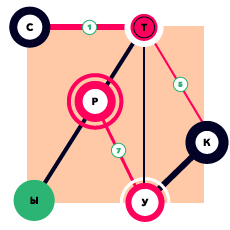
\includegraphics[scale=0.5]{Дискретные структуры картинка.png}
\caption{Эмблема дискретных структур.} \label{эмблема ДС}
\end{figure}

На рис.~\ref{эмблема ДС} можно ссылаться. 

Подрисунки можно добавлять с использованием subfigure, но для того, чтобы это окружение работало, в main надо кроме прочего добавить subcaption. Обратите внимание: несмотря на то, что вставлена фотография, контраста с белым фоном нет. Вам при фотографировании также нужно озаботиться тем, чтобы он не возникал (фотографировать сканером, а не стандартно).
\begin{figure}[H]
\centering
\begin{subfigure}[b]{0.45\linewidth}
\centering
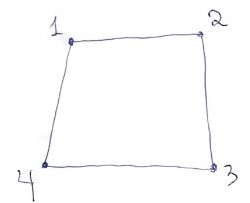
\includegraphics[scale=0.6]{Fall/img/Cycle-1.png}
\caption{Первый цикл} \label{цикл-1}
  \end{subfigure} 
  \begin{subfigure}[b]{0.45\linewidth} 
  \centering
  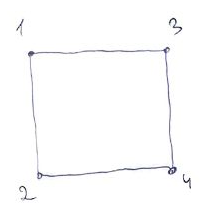
\includegraphics[scale=0.6]{Fall/img/Cycle-2.png}
  \caption{Второй цикл} \label{цикл-2}
  \end{subfigure}
 \caption{Два различных цикла.} \label{delta gamma = 2}
\end{figure}

На рис.~\ref{цикл-1} и~\ref{цикл-2} изображены два различных цикла.

Пример таблицы. Окружение \verb'array' необходимо заключать в пару \verb'$..$' для математических формул.
\begin{table}[H]
\centering
$
\begin{array}{|c|c|c|c|c|c|}
	\hline
	\text{Формула} & (1) & (2) & (3) & (4) & (13)\\
	\hline
	\exp\Gamma(\varphi^T) & 123202 & 702 & 4202 & 702 & 16\\
	\hline
\end{array}
$
\caption{Формула.} \label{таблица с формулой}
\end{table}
    




\begin{task}{441}
Перечислите все попарно неизоморфные связные простые графы на \(8\) вершинах, в которых ровно три блока и при этом не более двух простых циклов. Подробно описывать перебор не нужно (не нужно описывать получение каждого отдельного графа), но обязательно стоит разделить графы на группы по значениям параметров, по которым осуществлялся перебор (параметров должно быть минимум два, второй из которых позволяет перебирать графы с одинаковым значением первого параметра). При переборе случаев используйте вложенные окружения \textbf{enumerate} и окружение \textbf{figure}, не забудьте также использовать пары команд \textbf{ref} и \textbf{label} для описания рисунков. Описание случаев перебора должно происходить в тексте решения в tex-файле, а не внутри рисунков!
\end{task}

\begin{solution}

Будем пользоваться следующими определением и теоремой:

\begin{definition}\label{определение блок}
Блок~--- это максимальный подграф графа, не имеющий собственных точек сочленения (другими словами, некоторые точки сочленения графа могут принадлежать блоку, но своих точек сочленения у блока нет).
\end{definition}

\begin{theorem}\label{теорема цикл вершин блока}
В блоке с не менее чем тремя вершинами любые две из них связаны простым циклом.
\end{theorem}
\begin{proof}
Во-первых, заметим, что, если количество вершин в блоке меньше трех, цикла в нем быть не может.

Далее рассмотрим две вершины блока: $u$ и $v$. Обозначим $d(u,~v)$ как кратчайшее расстояние между ними.
\begin{enumerate}
    \item \label{$d(u,v)=1$} Если $d(u,~v) = 1$, значит, вершины смежны, причем ребро $(u,~v)$ не мост, иначе одна из вершин окажется точкой сочленения, что противоречит определению~\ref{определение блок}. Тогда существует простой цикл, проходящий через ребро $(u,~v)$, ведь при его удалении всё равно найдется цепь, соединяющая вершины $u$ и $v$.
    \item Пусть теперь $d(u,~v) > 1$. Возьмем кратчайший путь из $u$ в $v$, обозначив за $t$ предпоследнюю вершину этого пути. Тогда получим $d(u,~t) = d(u,~v) - 1$.
    
    Воспользуемся методом математической индукции и предположим, что уже существует простой цикл $C$, содержащий вершины $u$ и $t$.
    
    Так как $d(t,~v) = 1$, из п.~\ref{$d(u,v)=1$} получаем, что $t$ не точка сочленения, значит, есть простой путь $P$, соединяющий вершины $u$ и $v$ и не проходящий через $t$. Пусть $w$~--- первая вершина пути $P$ из $v$ в $u$, которая принадлежит $C$ (она точно существует, потому что $u \in C$). Получаем цикл, состоящий из:
    \begin{enumerate}
        \item части пути $P$ из $v$ в $w$;
        \item части цикла $C$ из $w$ в $t$, проходящей через $u$;
        \item ребра $(t,~v)$.
    \end{enumerate}
\end{enumerate}

\begin{figure}[H]
    \centering
    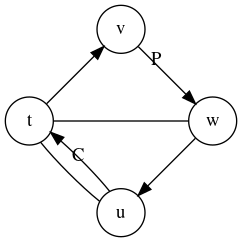
\includegraphics[scale=0.5]{Fall/img/solution-441_cycle_for_the_theorem.dot.png}
    \caption{Иллюстрация к доказательству теоремы (стрелками показан цикл).} \label{cycle for the theorem}
\end{figure}

База индукции уже установлена в п.~\ref{$d(u,v)=1$}, а также доказан переход: при предположении существования простого цикла, содержащего вершины $u$ и $t$, существует простой цикл, содержащий вершины $u$ и $v$, причем $d(u,~t) = d(u,~v) - 1$. Теорема доказана.
\end{proof}

Заметим, что граф на \(8\) вершинах должен содержать ровно три блока, значит, он имеет ровно две точки сочленения, условно разделяющих граф на блоки.

Теперь рассмотрим структуру блоков более подробно. Во-первых, необходимо

\begin{proposition}\label{k-цикл}
Если в блоке, содержащем $n$ вершин, есть простой цикл, содержащий меньшее количество вершин, то в блоке есть как минимум три различных простых цикла.
\end{proposition}
\begin{proof}
Занумеруем шаги наших рассуждений:
\begin{enumerate}
    \item Блок, содержащий три вершины, единственен: он должен быть полным, иначе одна из вершин окажется точкой сочленения, что противоречит определению~\ref{определение блок}.
    
    \item Допустим, при $n > 3$ нас есть $n$-блок, в котором есть цикл содержащий $k < n$ вершин (для удобства занумеруем их числами от \(1\) до \(k\)). Так как граф связный, остальные вершины с номерами от $k + 1$ до $n$ должны быть связаны с циклом, причем как минимум две из этих вершин точно должны иметь ребра, связывающие их с $k$-циклом, ведь в противном случае либо граф перестанет быть связным (ни одна из вершин с номерами, большими $k$ не связана с циклом ребром), либо найдется точка сочленения, что противоречит определению~\ref{определение блок} (одна вершина $x$ связана с вершиной цикла $y$ ребром, а остальные связаны с $x$ и/или между собой~--- тогда $y$ станет точкой сочленения).
    
    Получили, что как минимум две вершины связаны с $k$-циклом.
    
    \item Пусть у нас есть группа связанных между собой вершин $G$.
    
    \begin{enumerate}
        \item Если $|G| = 1$, другими словами, там только одна вершина $u$, значит, она должна быть связана как минимум двумя  ребрами с вершинами $k$-цикла (пусть это, условно, будут вершины $a$ и $b$). Тогда у нас есть минимум три цикла: ребра $(a,~u), (u,~b)$ и путь, соединяющий по циклу вершины $b$ и $a$; ребра $(a,~u), (u,~b)$ и путь, соединяющий по циклу вершины $a$ и $b$ (здесь уже берем другую часть цикла); исходный $k$-цикл.
        
        \begin{figure}[H]
            \centering
            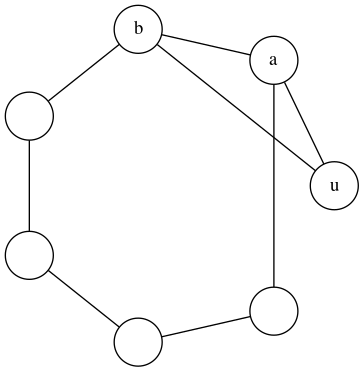
\includegraphics[scale=0.4]{Fall/img/solution-441_for_the_proposition.dot.png}
            \caption{Иллюстрация к доказательству утверждения $(a)$.} \label{cycle for the theorem b}
        \end{figure}
        
        \item Если же $|G| > 1$, то в ней найдется две вершины $u$ и $v$, соединенные с $k$-циклом ребрами, а также между собой. Рассуждения по нахождению трех циклов аналогичные, но уже с использованием пути, соединяющего $u$ и $v$ и не содержащего ребер $k$-цикла.
    \end{enumerate}
    
    С учетом существования $k$-цикла имеем минимум три уникальных цикла внутри блока. Значит при наличии в $n$-блоке $k$-цикла ($k < n$), в нём будут как минимум три цикла.
\end{enumerate}
\end{proof}

По утверждению~\ref{k-цикл} в $n$-блоке должен быть только $n$-цикл! А для любого $n > 2$ найти такие блоки~--- тривиальная задача. По сути мы получаем простое <<кольцо>> $n$ ребер, соединяющих $n$ вершин. Кстати говоря, это также означает, что каждый блок на $n > 3$ вершинах содержит ровно один цикл!

Так как по условию должно быть ровно три блока и не более двух циклов, а из теоремы~\ref{теорема цикл вершин блока} любой блок, содержащий не менее трех вершин, также содержит и цикл, получаем, что как минимум один из наших блоков должен состоять из двух вершин, другими словами, должен быть мостом (обе его вершины~--- точки сочленения). Также по утверждению~\ref{k-цикл} два других блока дадут нам необходимые два или менее цикла. Осталось перебрать тройки блоков: за параметр мы возьмем количество вершин в каждом из них. Исключая симметрию (например, тройки блоков $(2,~3,~5)$ и $(5,~3,~2)$ изоморфны), получаем семь вариантов, перечисленных на рисунках:
\begin{table}[H]
\centering
$
\begin{array}{|c|c|c|c|c|c|c|c|}
	\hline
	\text{Блок} & (2,~3,~5) & (2,~5,~3) & (2,~2,~6) & (2,~6,~2) & (3,~2,~5) & (2,~4,~4) & (4,~2,~4)\\
	\hline
	\text{Рисунок} & \ref{group 2-3-5} & \ref{group 2-5-3} & \ref{group 2-2-6} & \ref{group 2-6-2} & \ref{group 3-2-5} & \ref{group 2-4-4} & \ref{group 4-2-4}\\
	\hline
\end{array}
$
\caption{Ссылки на рисунки.} \label{groups refs}
\end{table}

Но и это еще не все! Две точки сочленения могут располагаться друг от друга на разном расстоянии в случае, когда средний блок имеет $n \geqslant 4$ вершин. Получаем как раз-таки два параметра поиска неизоморфных графов: количество вершин в тройке блоков, кратчайшее расстояние между точками сочленения. Изобразим итоговые варианты на рисунках (если $a, b, c$~--- количество вершин в трёх блоках, а $d$~--- кратчайшее расстояние между точками сочленения:

% (2, 3, 5) --- 1
\begin{figure}[H]
    \centering
    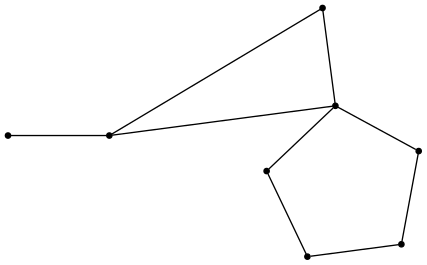
\includegraphics[scale=0.4]{Fall/img/solution-441_235_0.dot.png}
    \caption{Граф 2-3-5} \label{group 2-3-5}
\end{figure}

% (2, 5, 3) --- 3
\begin{figure}[H]
    \centering
    \begin{subfigure}[b]{0.45\linewidth}
        \centering
        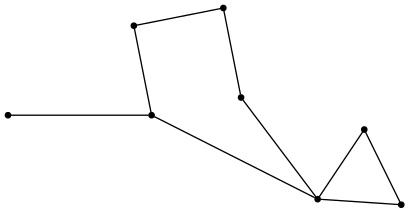
\includegraphics[scale=0.4]{Fall/img/solution-441_253_1.dot.png}
        \caption{Граф 2-5-3.1} \label{graph 2-5-3.1}
    \end{subfigure}
    \begin{subfigure}[b]{0.45\linewidth} 
        \centering
        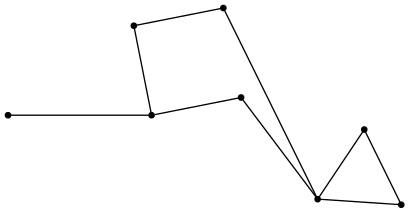
\includegraphics[scale=0.4]{Fall/img/solution-441_253_2.dot.png}
        \caption{Граф 2-5-3.2} \label{graph 2-5-3.2}
    \end{subfigure}
    \begin{subfigure}[b]{0.45\linewidth} 
        \centering
        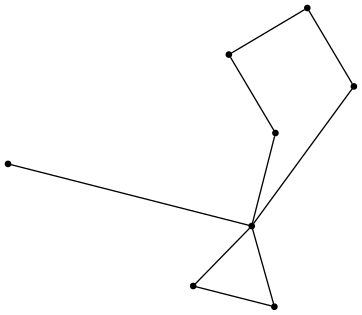
\includegraphics[scale=0.4]{Fall/img/solution-441_253_3.dot.png}
        \caption{Граф 2-5-3.3} \label{graph 2-5-3.3}
    \end{subfigure}
    
    \caption{Графы 2-5-3} \label{group 2-5-3}
\end{figure}

% (2, 2, 6) --- 1
\begin{figure}[H]
    \centering
    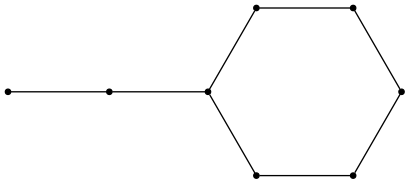
\includegraphics[scale=0.4]{Fall/img/solution-441_226_0.dot.png}
    \caption{Граф 2-2-6} \label{group 2-2-6}
\end{figure}

% (2, 6, 2) --- 4
\begin{figure}[H]
    \centering
    \begin{subfigure}[b]{0.45\linewidth}
        \centering
        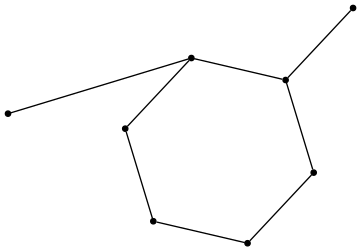
\includegraphics[scale=0.4]{Fall/img/solution-441_262_1.dot.png}
        \caption{Граф 2-6-2.1} \label{graph 2-6-2.1}
    \end{subfigure}
    \begin{subfigure}[b]{0.45\linewidth}
        \centering
        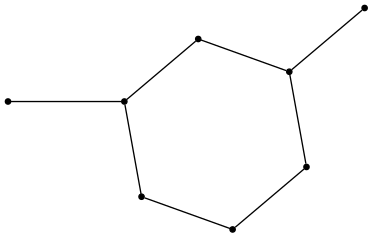
\includegraphics[scale=0.4]{Fall/img/solution-441_262_2.dot.png}
        \caption{Граф 2-6-2.2} \label{graph 2-6-2.2}
    \end{subfigure}
    \begin{subfigure}[b]{0.45\linewidth} 
        \centering
        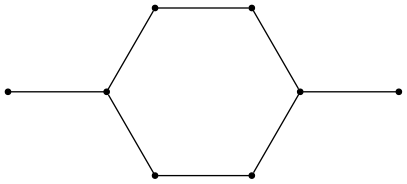
\includegraphics[scale=0.4]{Fall/img/solution-441_262_3.dot.png}
        \caption{Граф 2-6-2.3} \label{graph 2-6-2.3}
    \end{subfigure}
    \begin{subfigure}[b]{0.45\linewidth} 
        \centering
        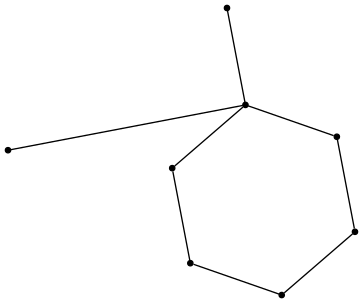
\includegraphics[scale=0.4]{Fall/img/solution-441_262_4.dot.png}
        \caption{Граф 2-6-2.4} \label{graph 2-6-2.4}
    \end{subfigure}
    
    \caption{Графы 2-6-2} \label{group 2-6-2}
\end{figure}

% (3, 2, 5) --- 1
\begin{figure}[H]
    \centering
    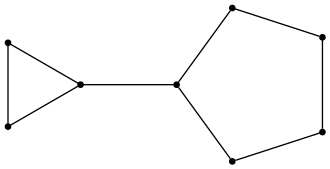
\includegraphics[scale=0.4]{Fall/img/solution-441_325_0.dot.png}
    \caption{Граф 3-2-5} \label{group 3-2-5}
\end{figure}

% (2, 4, 4) --- 3
\begin{figure}[H]
    \centering
    \begin{subfigure}[b]{0.45\linewidth}
        \centering
        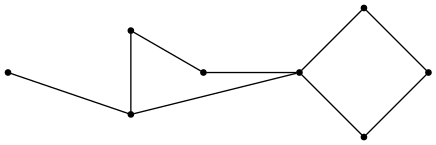
\includegraphics[scale=0.4]{Fall/img/solution-441_244_1.dot.png}
        \caption{Граф 2-4-4.1} \label{graph 2-4-4.1}
    \end{subfigure}
    \begin{subfigure}[b]{0.45\linewidth} 
        \centering
        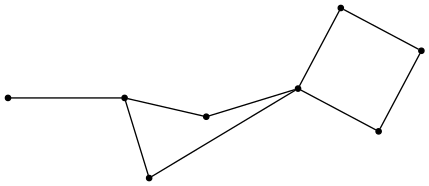
\includegraphics[scale=0.4]{Fall/img/solution-441_244_2.dot.png}
        \caption{Граф 2-4-4.2} \label{graph 2-4-4.2}
    \end{subfigure}
    \begin{subfigure}[b]{0.45\linewidth} 
        \centering
        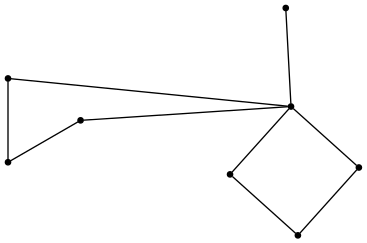
\includegraphics[scale=0.4]{Fall/img/solution-441_244_3.dot.png}
        \caption{Граф 2-4-4.3} \label{graph 2-4-4.3}
    \end{subfigure}
    
    \caption{Графы 2-4-4} \label{group 2-4-4}
\end{figure}

% (4, 2, 4) --- 1
\begin{figure}[H]
    \centering
    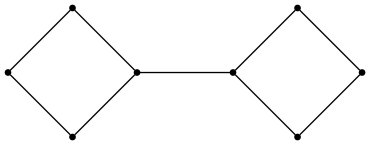
\includegraphics[scale=0.4]{Fall/img/solution-441_424_0.dot.png}
    \caption{Граф 4-2-4} \label{group 4-2-4}
\end{figure}

\textbf{Ответ:} Всего получаем 14 графов!

\end{solution}

\newpage
\begin{task}{455}
Сколькими способами можно расставить числа от \(1\) до \(15\) по кругу так, чтобы никакая пятерка чисел с одинаковым остатком по модулю \(3\) не стояла рядом (четыре числа с одинаковым остатком, соседствующие друг с другом, допустимы, а вот все пять — нет)? При этом расстановки считайте одинаковыми, если они получаются друг из друга циклическими сдвигами.
\end{task}

\begin{solution}

\begin{enumerate}
    \item Найдем общее число перестановок $\displaystyle K = \frac{15!}{15} = 14!$, так как циклические сдвиги считаются одинаковыми.
    
    \item Пусть $S_i$ --- количество перестановок, в которых числа с остатком $i$ стоят рядом и образуют пятерку. Найдем $K_1, K_2, K_3$:
    \begin{align*}
        K_1 &= \sum_{i=0}^{2} |S_i| = C_3^1 \cdot 5! \cdot 10!, \\
        K_2 &= \sum_{i<j} |S_i \cap S_j| = C_3^2 \cdot 5!^2 \cdot 6 \cdot 5!, \\
        K_3 &= |S_0 \cap S_1 \cap S_2| = C_3^3 \cdot 5!^3 \cdot 2.
    \end{align*}
    
    Здесь число сочетаний определяет, по какому модулю мы выбрали пятерки чисел; $(5!)^i$~--- перестановки внутри пятерок. Оставшиеся слагаемые определены так:
    \begin{enumerate}
        \item \textbf{Случай $K_1$:} $10!$ --- это перестановки остальных элементов;
        
        \item \textbf{Случай $K_2$:} \(6\) отвечает за варианты положения второй пятерки относительно первой, $5!$ --- за перестановки остальных элементов;
        
        \item \textbf{Случай $K_3$:} \(2\) отвечает за уникальные комбинации пятерок. Всего их может быть шесть (числами обозначены общие для пятерок остатки при делении на три):
        \begin{equation*}
            (0, 1, 2), (0, 2, 1), (1, 0, 2), (1, 2, 0), (2, 0, 1), (2, 1, 0),
        \end{equation*}
        из которых остается только две уникальные: $(0,~1,~2), (0,~2,~1)$.
    \end{enumerate}
    
    По формуле включений-исключений получаем:
    \begin{multline*}
        |K \backslash (S_0 \cup S_1 \cup S_2)| = |K| - |K_1| + |K_2| - |K_3| = \\
        = 14! - C_3^1 \cdot 5! \cdot 10! + C_3^2 \cdot 5!^2 \cdot 6 \cdot 5! - C_3^3 \cdot 5!^3 \cdot 2 = \\
        = 14! - 5!^2 \cdot \left( 3 \cdot \left( 6 \cdot 7 \cdot 8 \cdot 9 \cdot 10 \right) - 3 \cdot 6 \cdot 5! + 5! \cdot 2 \right) = \\
        = 14! - 5!^3 \cdot (6 \cdot 7 \cdot 9 \cdot 2 - 3 \cdot 6 + 2) = 14! - 5!^3 \cdot \left( 756 - 18 + 2 \right) = \\
        = 14! - 5!^3 \cdot 740 = 14! - 5!^3 \cdot 4 \cdot 5 \cdot 37 = 85899571200.
    \end{multline*}
\end{enumerate}

\textbf{Ответ:} 85899571200.

\end{solution}

\begin{task}{460}
Выведите явную формулу для числа неупорядоченных разбиений \(p_3(n)\) для произвольного \(n\). Ответ не должен являться рекуррентной формулой, но при этом разрешено оставлять его в виде суммы с переменным (зависящим от \(n\)) числом слагаемых.
\end{task}

\begin{solution}

Для удобства воспользуемся представлением этой суммы в виде диаграммы Юнга. Вот пример представления \(n = 8\):

\begin{figure}[H]
    \centering
    \ytableausetup{centertableaux}
    \begin{ytableau}
        \none[3]    &       & \none & \none & \none & \none & \none \\
        \none[2]    &       &       &       & \none & \none & \none \\
        \none[1]    &       &       &       &       & \none & \none \\
        \none       & \none[1] & \none[2] & \none[3] & \none[4] & \none[5] & \none[6]
    \end{ytableau}
    \caption{Диаграмма Юнга: пример разбиения при \(n = 8\).} \label{example_diagram_460}
\end{figure}

На рис.~\ref{example_diagram_460} отмечены три слагаемых, и в строках значение каждого из них представлено <<кубиками>>, число которых не превышает \(n - 2\). Почему именно такое ограничение на значение слагаемого? По условию задачи их обязательно должно быть три, значит, каждый из них не может быть нулевым, поэтому хотя бы один <<кубик>> у каждого слагаемого должен быть. Остается разместить \(n - 3\) <<кубиков>>. Чтобы найти максимальное значение слагаемого, поместим их все в одну ячейку, допустим, в третью. Тогда значение третьего слагаемого будет равно \(n - 2\). Больше быть не может:

\begin{figure}[H]
    \centering
    \ytableausetup{centertableaux}
    \begin{ytableau}
        \none[3]    &       & \none & \none & \none & \none & \none \\
        \none[2]    &       & \none & \none & \none & \none & \none \\
        \none[1]    &       &       &       &       &       &       \\
        \none       & \none[1] & \none[2] & \none[3] & \none[4] & \none[5] & \none[6]
    \end{ytableau}
\end{figure}

Обозначим \(a_1, a_2, a_3\) за три слагаемых, сумма которых равна \(n\). Попробуем отыскать количество решений уравнения \(a_1 + a_2 + a_3 = n\), рассуждая следующим образом:
\begin{enumerate}
    \item Нужно найти количество неупорядоченных разбиений. Два решения считаются эквивалентными, если они одинаковы с точностью до перестановок слагаемых. Тогда расположим слагаемые в порядке возрастания: \(a_1 \leqslant a_2 \leqslant a_3\);
    
    \item Слагаемых должно быть ровно три, значит, каждое из них ненулевое. Так мы определили нижнюю грань: \(1 \leqslant a_1 \leqslant a_2 \leqslant a_3\);
    
    \item Попробуем отыскать верхние грани для каждого из слагаемых:
    \begin{enumerate}
        \item Заметим, что, если \(a_1 = k\), то \(a_2, a_3 \geqslant k\). Тогда максимально возможное значение \(a_1\)~--- это \(\displaystyle \floor{\frac{n}{3}}\), ведь в противном случае сумма слагаемых превысит \(n\);
        
        \item Зафиксируем \(a_1 = k\). Тогда уравнение примет вид: \(a_2 + a_3 = n - k\). Аналогично рассуждениям предыдущего пункта выводим \(\displaystyle a_2 \leqslant \floor{\frac{n - k}{2}}\);
        
        \item Верхнюю грань \(a_3\) искать нет смысла, потому что оно зависит от выбора подходящих \(a_1, a_2\). Однако это было сделано выше при описании рис.~\ref{example_diagram_460}: \(a_3 \leqslant n - 2\).
    \end{enumerate}
\end{enumerate}

Наш ответ теперь можно явно получить перебором:
\begin{equation*}
    S_{3}(n) = \mathlarger{\sum_{k = 1}^{\floor{\frac{n}{3}}} \sum_{m = k}^{\floor{\frac{n - k}{2}}} 1} =
    \sum_{k = 1}^{\floor{\frac{n}{3}}} \left( \floor{\frac{n - k}{2}} - k + 1 \right).
\end{equation*}

\textbf{Ответ:} \(\displaystyle S_{3}(n) = \sum_{k = 1}^{\floor{\frac{n}{3}}} \left( \floor{\frac{n - k}{2}} - k + 1 \right)\).

\end{solution}

\begin{task}{461}
Найдите сумму количеств неупорядоченных разбиений натуральных чисел \(2\leqslant n\leqslant 57\), таких, что каждое разбиение состоит не более, чем из \(10\) слагаемых и максимальное слагаемое в каждом из которых не больше \(6\).
\end{task}

\begin{solution}

Для удобства воспользуемся представлением этой суммы в виде диаграммы Юнга. Вот пример представления \(n = 28\):

\begin{figure}[H]
    \centering
    \ytableausetup{centertableaux}
    \begin{ytableau}
        \none[10]   & \none & \none & \none & \none & \none & \none \\
        \none[9]    & \none & \none & \none & \none & \none & \none \\
        \none[8]    &       & \none & \none & \none & \none & \none \\
        \none[7]    &       & \none & \none & \none & \none & \none \\
        \none[6]    &       &       & \none & \none & \none & \none \\
        \none[5]    &       &       &       & \none & \none & \none \\
        \none[4]    &       &       &       &       &       & \none \\
        \none[3]    &       &       &       &       &       & \none \\
        \none[2]    &       &       &       &       &       & \none \\
        \none[1]    &       &       &       &       &       &       \\
        \none       & \none[1] & \none[2] & \none[3] & \none[4] & \none[5] & \none[6]
    \end{ytableau}
    \caption{Диаграмма Юнга: пример разбиения при \(n = 28\).} \label{example_diagram_461}
\end{figure}

На рис.~\ref{example_diagram_461} отмечены \(10\) слагаемых, и в строках значение каждого из них представлено <<кубиками>>, число которых не превышает шести, что соответствует условию задачи. Заметим также, что, если слагаемое равно нулю, <<кубиков>> у него нет и мы считаем, что в разбиении этого слагаемого не существует. Так рис.~\ref{example_diagram_461} можно представить в виде суммы:
\begin{equation*}
    28 = 6 + 5 + 5 + 5 + 3 + 2 + 1 + 1.
\end{equation*}

Указано \(8\) слагаемых, так как два слагаемых в разбиении являются нулями. Условие о том, что каждое разбиение состоит не более, чем из \(10\) слагаемых, также соблюдено.

Представим возможные значения слагаемых <<ящиками>> (от нуля до шести), в которые распределим сами слагаемые~--- <<шары>>. Нам нужна неупорядоченная выборка, в которой значения могут повторяться~--- это число сочетаний с повторениями. Имеем:
\begin{equation*}
    \overline C_{7}^{10} = C_{7 + 10 - 1}^{10} = C_{16}^{10} = \frac{16!}{10!(16 - 10)!} = 8008.
\end{equation*}

Так мы перебрали все представления \(0\leqslant n\leqslant 60\). Однако по условию \(2\leqslant n\leqslant 57\), значит, мы должны исключить варианты:
\begin{enumerate}
    \item \(n = 0\). Его представление единственно: все слагаемые равны нулю, точнее сказать, их вообще нет;
    \item \(n = 1\). Его представление единственно: единственное слагаемое, равное \(1\) (остальные~--- нули);
    \item \(n = 58\). Найдется всего лишь два варианта неупорядоченного разбиения:
        \begin{figure}[H]
            \centering
            \begin{subfigure}[b]{0.45\linewidth}
                \centering
                \ytableausetup{centertableaux}
                \begin{ytableau}
                    \none[10]   &       &       &       &       & \none & \none \\
                    \none[9]    &       &       &       &       &       &       \\
                    \none[8]    &       &       &       &       &       &       \\
                    \none[7]    &       &       &       &       &       &       \\
                    \none[6]    &       &       &       &       &       &       \\
                    \none[5]    &       &       &       &       &       &       \\
                    \none[4]    &       &       &       &       &       &       \\
                    \none[3]    &       &       &       &       &       &       \\
                    \none[2]    &       &       &       &       &       &       \\
                    \none[1]    &       &       &       &       &       &       \\
                    \none       & \none[1] & \none[2] & \none[3] & \none[4] & \none[5] & \none[6]
                \end{ytableau}
                \caption{Диаграмма Юнга: \(n = 58\).} \label{young_diagram_58_1}
            \end{subfigure}
            \begin{subfigure}[b]{0.45\linewidth}
                \centering
                \ytableausetup{centertableaux}
                \begin{ytableau}
                    \none[10]   &       &       &       &       &       & \none \\
                    \none[9]    &       &       &       &       &       & \none \\
                    \none[8]    &       &       &       &       &       &       \\
                    \none[7]    &       &       &       &       &       &       \\
                    \none[6]    &       &       &       &       &       &       \\
                    \none[5]    &       &       &       &       &       &       \\
                    \none[4]    &       &       &       &       &       &       \\
                    \none[3]    &       &       &       &       &       &       \\
                    \none[2]    &       &       &       &       &       &       \\
                    \none[1]    &       &       &       &       &       &       \\
                    \none       & \none[1] & \none[2] & \none[3] & \none[4] & \none[5] & \none[6]
                \end{ytableau}
                \caption{Диаграмма Юнга: \(n = 58\).} \label{young_diagram_58_2}
            \end{subfigure}
            \caption{Диаграмма Юнга: два варианта разбиения при \(n = 58\).} \label{young_diagram_58}
        \end{figure}
    \item \(n = 59\). Его представление единственно: все слагаемые равны \(6\), кроме одного со значением \(5\);
    \item \(n = 60\). Его представление единственно: все слагаемые равны \(6\).
\end{enumerate}

Значит, исключаем \(6\) лишних разбиений. И получаем \textbf{ответ}:
\begin{equation*}
    \overline C_{7}^{10} - 6 = 8008 - 6 = 8002.
\end{equation*}

\end{solution}

\begin{task}{47}
Сколько существует различных помеченных унициклических графов на ровно \(n\) вершинах с циклом длины \(7\)? Считайте, что \(n\geqslant 9\).
\end{task}

\begin{solution}

\begin{enumerate}
    \item Унициклический граф:
    \begin{enumerate}
        \item имеет один цикл;
        \item является связным.
    \end{enumerate}
    А так как по условию задачи нужен такой граф с циклом длины \(7\), выберем \(7\) помеченных вершин и обозначим их множество как \(\dot{V}\).
    
    \item Найдем число способов \(\dot{C}\) выбрать цикл длины \(7\) среди \(n\) помеченных вершин:
    \begin{enumerate}
        \item Количество способов отобрать последовательности типа \(\overline{1234567}: C_{n}^{7}\);
        \item Учтем перестановки внутри последовательностей: \(7!\);
        \item Например, циклы \(\overline{1234567}, \overline{2345671}\) и \(\overline{7654321}\) являются эквивалентными (7 сдвигов и обратная запись). Значит, конечный ответ следует разделить на \(7 \cdot 2\);
    \end{enumerate}
    В итоге получаем:
    \begin{equation*}
        \dot{C} = C_{n}^{7} \cdot \frac{7!}{7 \cdot 2}.
    \end{equation*}
    
    \item Цикл нашли! Оставшиеся вершины будем <<цеплять>> за все \(v \in \dot{V}\) так, чтобы новых циклов не получилось~--- значит, это будут деревья. Сам граф же становится лесом с \(7\) компонентами.
    
    \item Помним, что количество помеченных лесов на \(n\) вершинах с \(r\) компонентами, каждая из
которых содержит ровно по одной вершине из множества \(\{1, \ldots, r\}\), в точности \(rn^{n - 1 - r}\) штук. В условиях нашей задачи \(r \equiv 7\).

    \item Как итог, количество \(\dot{P}\) помеченных унициклических графов на \(n\) вершинах с циклом длины \(7\):
    \begin{multline*}
        \dot{P} = \dot{C} \cdot 7 \cdot n^{n - 1 - 7} = C_{n}^{7} \cdot \frac{7!}{7 \cdot 2} \cdot 7 \cdot n^{n - 1 - 7} = \\
        = \frac{n!}{7!(n - 7)!} \cdot \frac{7! \cdot 7 \cdot n^{n - 8}}{7 \cdot 2} = \frac{n!}{(n - 7)!} \cdot \frac{n^{n - 8}}{2} = A_{n}^{7} \cdot \frac{n^{n - 8}}{2}.
    \end{multline*}
\end{enumerate}

\textbf{Ответ:} \(\displaystyle \dot{P} = A_{n}^{7} \cdot \frac{n^{n - 8}}{2}\).

\end{solution}

\begin{task}{445}
Постройте \textbf{троичную} последовательность де Брёйна порядка три, начинающуюся с «\(012010\ldots\)». Сделайте это, найдя эйлеров цикл в соответствующем графе. Рисунок использованного для построения последовательности графа обязательно добавьте в решение, пронумеровав рёбра графа в порядке прохождения по эйлеровому циклу. Длина последовательности должна быть равна \(q^n+n-1\), где \(q\)~--- размер алфавита, а \(n\)~--- порядок последовательности.
\end{task}

\begin{figure}[H]
    \centering
    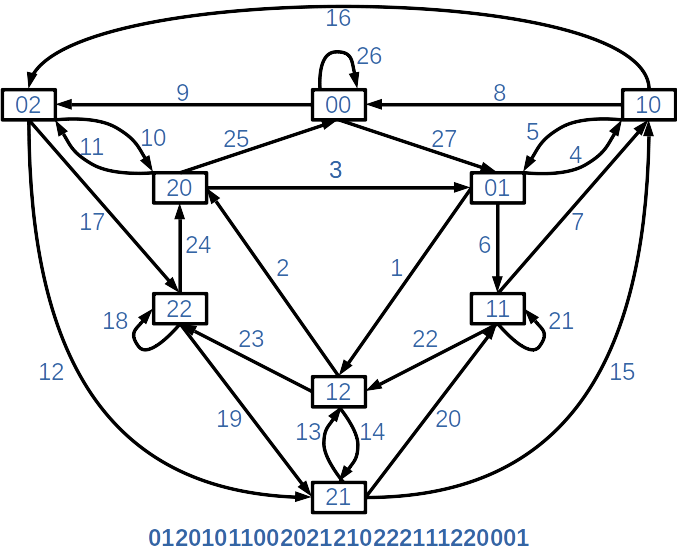
\includegraphics[scale=0.6]{Fall/img/solution-445_answer.png}
    \caption{Граф к задаче 445.} \label{graph 381}
\end{figure}

\textbf{Ответ:} 01201011002021210222111220001.

\newpage
\begin{task}{381}
Пусть ребра графа \(G\) правильно раскрашены в цвета \(\{0,1,2,\ldots,k\}\). Предположим, в \(G\) есть ровно одно ребро цвета \(0\), его концы~--- \(u,v\). Пусть также известно, что для покраски ребер, инцидентных \(u\), использованы все цвета, кроме \(k\), а для покраски ребер, инцидентных \(v\),~--- все, кроме \(1\) и \(2\). Пусть \(\{u,w\}\)~--- ребро цвета \(1\). Оказалось, что для раскраски ребер, инцидентных \(w\), не использованы цвета \(0\) и \(2\). Докажите, что ребра \(G\) можно правильно раскрасить в \(k\) цветов.  
\end{task}

Разложим условие <<по полочкам>>:
\begin{enumerate}
    \item Граф \(G\) правильно раскрашен в \((k + 1)\) цвет. А мы хотим получить правильную раскраску в \(k\) цветов. По условию существует только одно ребро цвета \(0\)~--- это ребро \((u, v)\). \textbf{Если получится убрать ребро с цветом \(0\), тогда мы добьемся цели}.
    
    \item В условии очень подробно расписаны цвета ребер, инцидентных вершинам \(u, v, w\). Представим это в виде небольшой схемы для удобства восприятия:
    \begin{figure}[H]
        \centering
        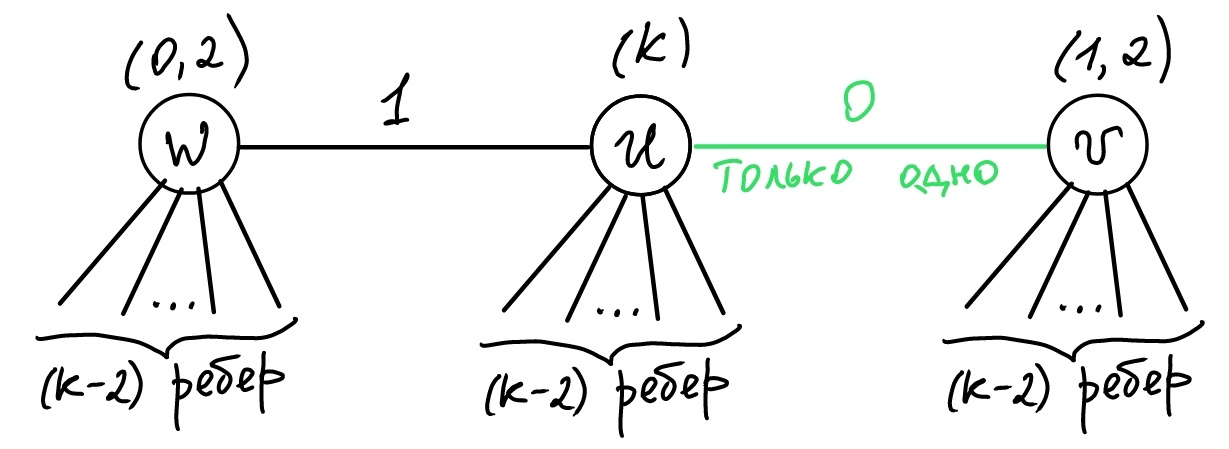
\includegraphics[scale=0.3]{Fall/img/solution-381_scheme.jpg}
        \caption{Условие в виде схемы.} \label{scheme 381}
    \end{figure}
    
    Далее будем пользоваться следующими обозначениями, часть которых изображена на схеме~\ref{scheme 381}:
    \begin{enumerate}
        \item Возле вершины в скобках будем показывать цвета, которые не встречаются среди цветов инцидентных ребер. Так по условию <<для покраски ребер, инцидентных \(u\), использованы все цвета, кроме \(k\)>>, значит, в скобках укажем только \(k\). Аналогично из условия возле вершины \(v\) указаны цвета \(1, 2\), возле вершины \(w\)~--- цвета \(0, 2\);
        
        \item Ребро, помеченное цветом \(0\) единственно. Далее будем обозначать его \emph{нуль-ребро}.
    \end{enumerate}
\end{enumerate}

Чтобы убрать \emph{нуль-ребро}, нужно в конечном счете пометить его каким-либо другим цветом. Сразу сделать это не получится, иначе нарушится условие правильной раскраски. Тогда введем операцию обмена цветами (\emph{swap}) у двух ребер, инцидентных одной вершине. И наложим важное ограничение, чтобы раскраска после обмена оставалась правильной:
\begin{figure}[H]
    \centering
    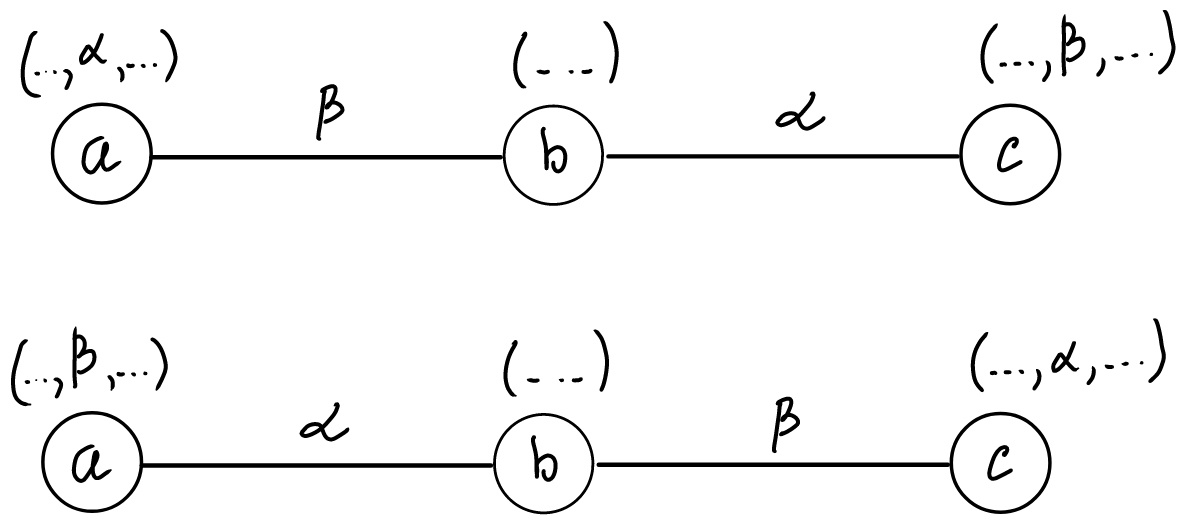
\includegraphics[scale=0.2]{Fall/img/solution-381_swap.jpg}
\end{figure}

Обмен цветами ребер \((a, b) \Leftrightarrow \beta\) и \((b, c) \Leftrightarrow \alpha\) сохранит условие правильной раскраски, если вершина \(a\) не имеет цвета \(\alpha\), а вершина \(c\) не имеет цвета \(\beta\).

\emph{Заметка:} мы будем использовать \emph{swap} только с \emph{нуль-ребром}, за цветом которого следить не нужно, потому что вершины, не инцидентные \emph{нуль-ребру}, гарантированно не будут иметь цвета \(0\).

Когда мы сможем заменить цвет \emph{нуль-ребра}? Когда возникнет ситуация, при которой обе вершины, соединенные \emph{нуль-ребром}, не будут иметь один и тот же цвет, допустим, цвет \(m\). Тогда заменяем цвет \(0\) на цвет \(m\) и побеждаем. Назовем эту ситуацию \textbf{Победа}.

Теперь другой вопрос: как добиться такой ситуации? Попробуем вовлечь в игру с обменами цвета, которые упомянуты в условии~--- это \(\{0, 1, 2, k\}\). А ребра с остальными цветами просто <<выкинем>>, потому что они ни на что не будут влиять.

Итак, мы получили граф с четырьмя цветами и хотим сделать так, чтобы осталось только три цвета. Стартуем с \emph{нуль-ребра} и начинаем двигаться по цепи вида \((0-k-2-k-\ldots-)\) в сторону вершины \(v\) и далее:
\begin{figure}[H]
    \centering
    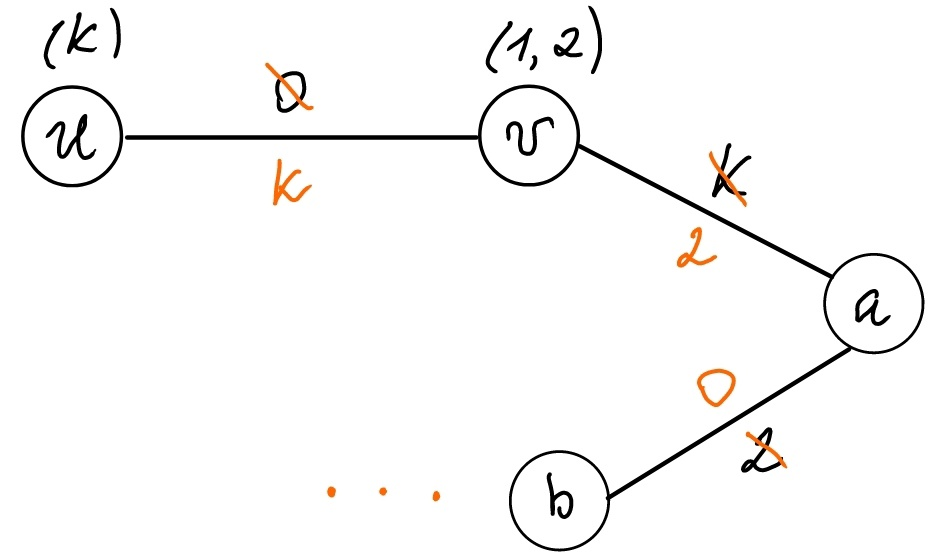
\includegraphics[scale=0.2]{Fall/img/solution-381_chain_begin.jpg}
\end{figure}

Если вдруг в процессе <<продвижения>> \emph{нуль-ребра} у вершины не окажется ребра цвета \(2\) после обмена \emph{ нуль-ребра} с ребром цвета \(k\), или наоборот~--- тогда алгоритм можно завершать, потому что мы пришли к ситуации \textbf{Победа}:
\begin{figure}[H]
    \centering
    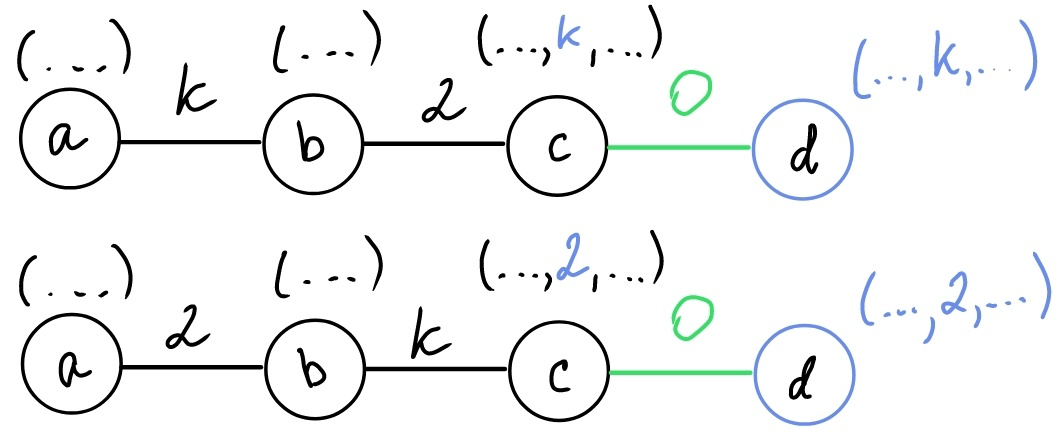
\includegraphics[scale=0.3]{Fall/img/solution-381_chain_end.jpg}
    \caption{Конец цепи, победа.} \label{chain win 381}
\end{figure}

Почему мы так смело утверждаем, что у вершины \(c\) нет цвета \(k\) или \(2\), необходимого для ситуации \textbf{Победа}~\eqref{chain win 381}? Дело в том, что при продвижении \emph{нуль-ребра} произошел <<сдвиг>> ребер с цветами \(2, k\), что привело к исчезновению одного из цветов у вершины \(c\). В первом случае от нее <<ушло>> ребро цвета \(k\:((b, c) \rightarrow (a, b))\); во втором~--- ребро цвета \(2\).

Но что если такой ситуации не случится? Бесконечной цепь быть не может, значит, она замкнется в стартовой вершине \(u\) и получится цикл:
\begin{figure}[H]
    \centering
    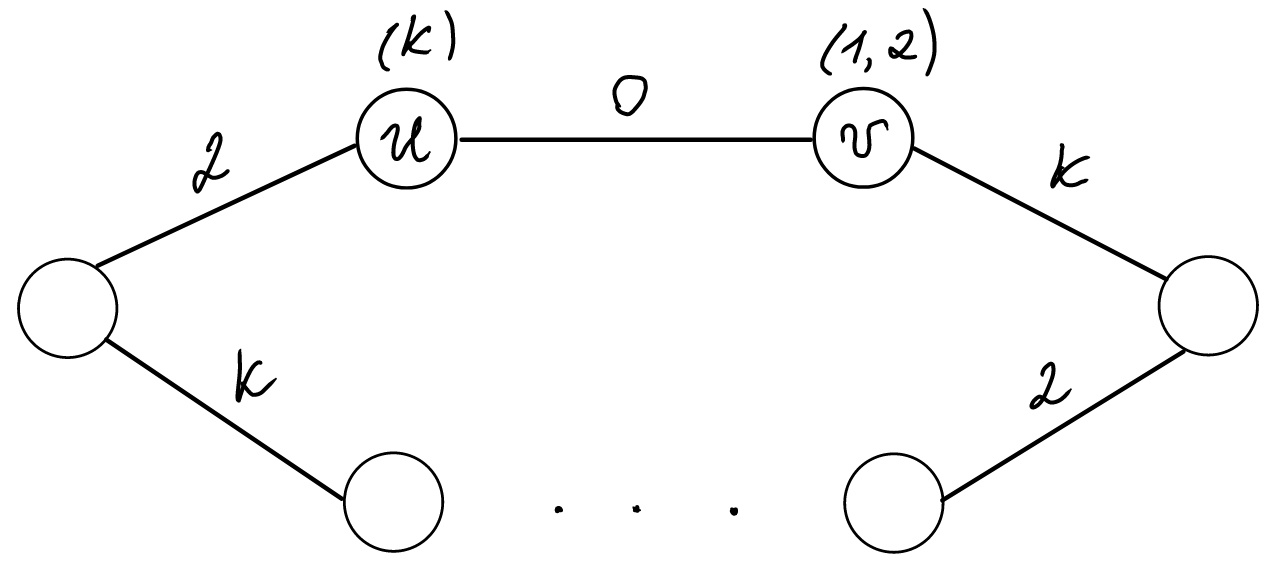
\includegraphics[scale=0.3]{Fall/img/solution-381_cycle.jpg}
    \caption{Цикл, включающий \emph{нуль-ребро} \((u, v)\)} \label{cycle 381}
\end{figure}

Это совсем не то, что нам нужно, ведь в цикле мы через какое угодно количество операций \emph{swap} не придем к ситуации \textbf{Победа}~\eqref{chain win 381}. Но и здесь мы можем извлечь выгоду. Допустим, что у нас не один такой цикл, а два: оба проходят через вершину \(u\); первый также проходит через вершину \(v\), второй, соответственно, через вершину \(w\); оба имеют общую часть \((u-t)\):
\begin{figure}[H]
    \centering
    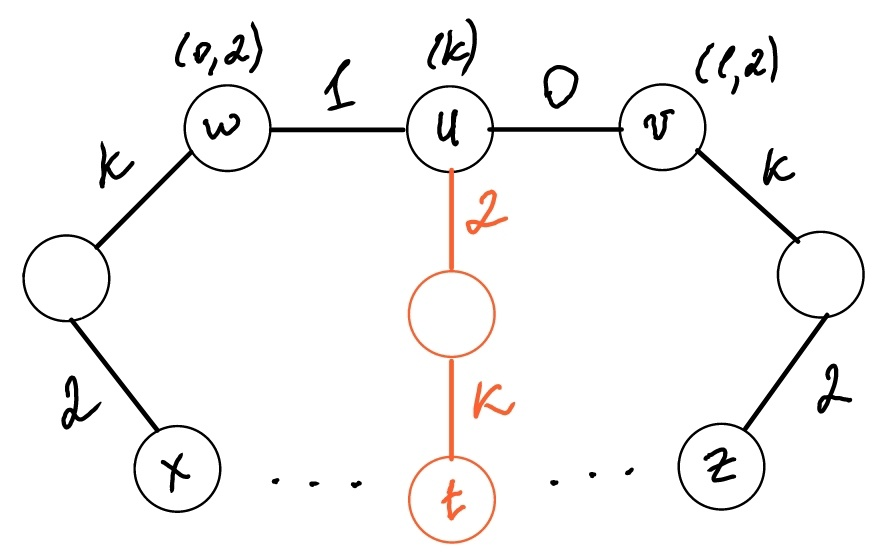
\includegraphics[scale=0.3]{Fall/img/solution-381_two_cycles.jpg}
    \caption{Два цикла быть не может.} \label{two cycles 381}
\end{figure}

Такая ситуация возможна? Нет! Ведь тогда каждый из циклов соединен с вершиной \(t\) ребром одного и того же цвета, другими словами, из вершины \(t\) исходят два ребра одного и того же цвета, а это противоречит правильности раскраски.

Используем это умозаключение. Допустим, образовался цикл~\ref{cycle 381}. Тогда если мы начнем обход из вершины \(u\), но уже через вершину \(w\), цепь замкнуть не сможем.

Но есть загвоздка: цепь \((u-w-\ldots-)\) не содержит \emph{нуль-ребра}. Эта проблема решается очень легко: сделаем \emph{swap} ребер \((u, v), (u, w)\). Это возможно, потому что \(u\) не содержит цвета \(1\), а \(w\) не содержит цвета \(0\). Более наглядно:
\begin{figure}[H]
    \centering
    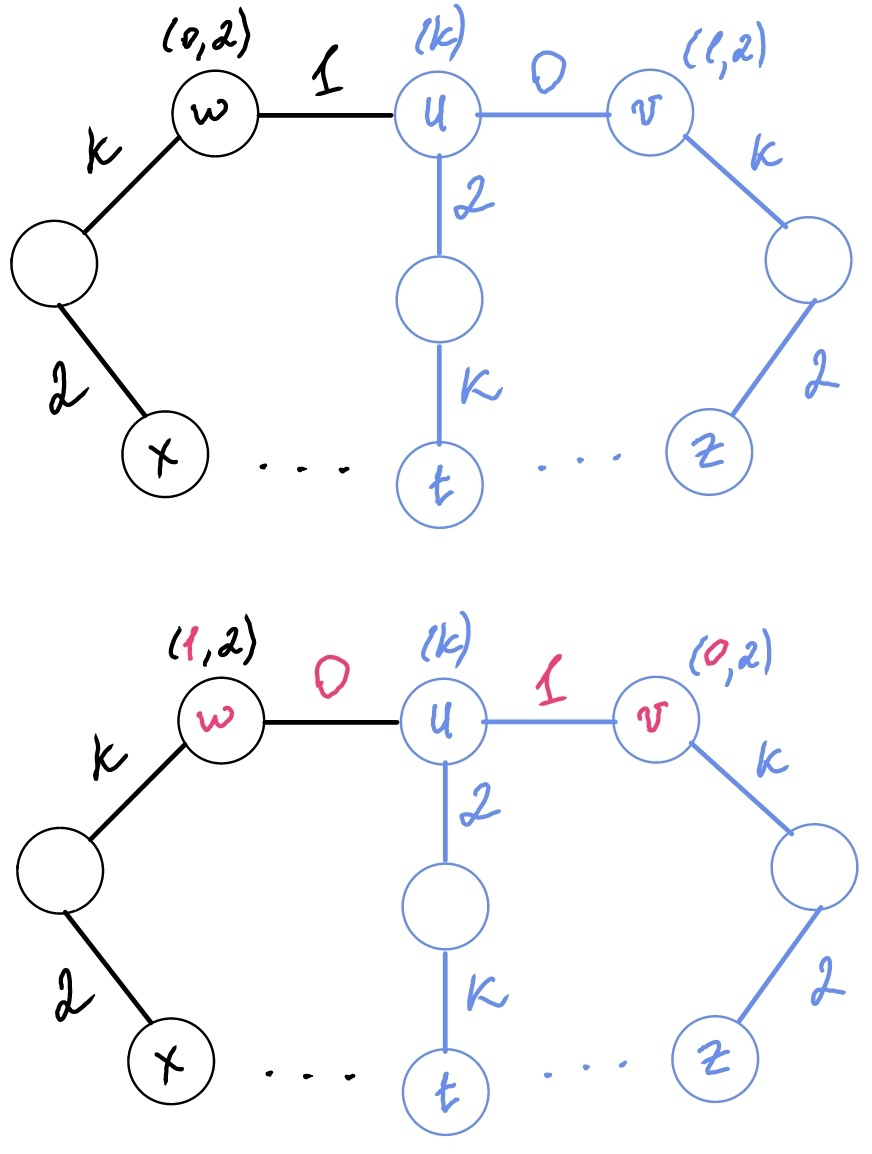
\includegraphics[scale=0.3]{Fall/img/solution-381_main_swap.jpg}
    \caption{Обмен ребер \((u, v), (u, w)\).} \label{main swap 381}
\end{figure}

Получаем цепь \((u-w-\ldots-)\), содержащую \emph{нуль-ребро}, которая никогда не замкнется, значит, обязательно придем к ситуации \textbf{Победа}~\eqref{chain win 381}~--- в противном случае цепь будет бесконечной.

\textbf{Коротко пробежимся по готовому плану:}

Нужно убрать \emph{нуль-ребро}. Для этого мы рассмотрели только ребра с цветами \(\{0, 1, 2, k\}\), потому что остальные не влияют на правильность раскраски по ходу алгоритма, ввели операцию \emph{swap} и приняли стратегию нахождения конечной цепи. Наша цель~--- ситуация \textbf{Победа}~\eqref{chain win 381}, при которой возможно изменение цвета \(0\) на любой другой с сохранением правильности раскраски. Дальше получаем несколько случаев:
\begin{enumerate}
    \item Цепь \((u-v-\ldots-)\) конечна. После серии операций \emph{swap} приходим к ситуации \textbf{Победа}~\eqref{chain win 381};
    
    \item Цепь \((u-v-\ldots-)\) замыкается~--- получаем цикл. Тогда:
    \begin{enumerate}
        \item Делаем \emph{swap} ребер \((u, v), (u, w)\) с сохранением правильности раскраски~\eqref{main swap 381};
        
        \item Рассматриваем всегда конечную цепь \((u-w-\ldots-)\), содержащую \emph{нуль-ребро}. После серии операций \emph{swap} приходим к ситуации \textbf{Победа}~\eqref{chain win 381}.
    \end{enumerate}
\end{enumerate}

После выполнения плана мы сохраняем правильность раскраски и перекрашиваем единственное ребро цвета \(0\) в один из цветов \(\{2, k\}\). Получаем искомую правильную раскраску графа \(G\) в \(k\) цветов.

\newpage
\begin{task}{283}
Ориентированный граф называется \textit{сильно связным}, если для любых двух его вершин \(s\) и \(t\) существует как ориентированный путь из \(s\) в \(t\), так и ориентированный путь из \(t\) в \(s\). Докажите, что в любом сильно связном турнире существует ориентированный гамильтонов цикл.
\end{task}

Будем рассматривать турниры, обозначив \(V\)~--- множество его вершин, \(E\)~--- множество его дуг и \(|V| \geqslant 3\). Докажем, используя метод математической индукции по числу вершин в цикле.

Для начала покажем, что в сильно связном турнире найдется цикл длины \(3\).

Выберем любую вершину \(v\). Так как турнир сильно связный, найдутся и входящие, и выходящие дуги~--- разделим их на два непересекающихся множества \(I\) и \(O\). Более формально:
\begin{align*}
    I &= \{i \in V\:\mid\:(i, v) \in E \},\\
    O &= \{o \in V\:\mid\:(v, o) \in E \}.
\end{align*}

Так как турнир сильно связный:
\begin{enumerate}
    \item \(I\) и \(O\) не пустые;
    
    \item Существует связывающее \(O\) и \(I\) дуга:
    \begin{equation*}
        \exists (i_1 \in I, o_1 \in O)\:\mid\:(o_1, i_1) \in E,
    \end{equation*}
    иначе не было бы пути из одного множества в другое.
\end{enumerate}

Наш искомый цикл (\(v - o_1 - i_1 - v\)) и его длины равна трем.

Теперь предположим, что в турнире есть простой цикл длины \(k < |V|\). Пусть это будет
\begin{equation*}
    C_k = (v_1 \rightarrow v_2 \rightarrow \ldots \rightarrow v_k \rightarrow v_1).
\end{equation*}

Так длины цикла меньше количества вершин турнира, \(\exists v_0 \in V, v_0 \notin C_k\). Возможны две ситуации:
\begin{enumerate}
    \item Существуют вершины цикла \(v_i, v_j\):
    \begin{equation*}
        \exists (v_i, v_0), (v_0, v_j) \in E;
    \end{equation*}
    
    \item Таких вершин \(v_i, v_j\) не нашлось.
\end{enumerate}

В первом случае мы обозначим за \(v_j\) \textbf{первую} вершину при обходе \(C_k\), для которой \(\exists (v_o, v_j) \in E\). Тогда вершина \(v_{j-1}\) такова, что \(\exists (v_{j-1}, v_o) \in E\). Она существует, так как существует входящая в \(v_0\) из цикла дуга. Тогда наш искомый цикл длины \(k + 1\):
\begin{equation*}
    (v_1 \rightarrow v_2 \rightarrow \ldots \rightarrow v_{j-1} \rightarrow v_0 \rightarrow v_j \rightarrow \ldots \rightarrow v_k \rightarrow v_1).
\end{equation*}

Заметим также, что, если в \(C_k\) не входит лишь одна вершина, образуется первая ситуация, иначе дуги \(v_0\) только входящие или только исходящие, что противоречит условию сильной связности.

Во втором случае мы разделяем вершины, не принадлежащие циклу \(C_k\) на два непересекающихся множества входящих в его вершины и выходящих из них:
\begin{align*}
    I_{C_k} &= \{x \in V \wedge x \notin C_k\:\mid\:(\forall v_i \in C_k)\:(x, v_i) \in E \},\\
    O_{C_k} &= \{y \in V \wedge y \notin C_k\:\mid\:(\forall v_i \in C_k)\:(v_i, y) \in E \}.
\end{align*}

Так как турнир сильно связный:
\begin{enumerate}
    \item \(I_{C_k}\) и \(O_{C_k}\) не пустые;
    
    \item Существует связывающее \(O_{C_k}\) и \(I_{C_k}\) дуга:
    \begin{equation*}
        \exists (i_2 \in I_{C_k}, o_2 \in O_{C_k})\:\mid\:(o_2, i_2) \in E,
    \end{equation*}
    иначе не было бы пути из одного множества в другое.
\end{enumerate}

Соответственно, наш искомый цикл длины \(k + 1\):
\begin{equation*}
    (v_1 \rightarrow o_2 \rightarrow i_2 \rightarrow v_3 \rightarrow \ldots \rightarrow v_k \rightarrow v_1).
\end{equation*}

В каждом из двух случаев находится цикл длины \(k + 1\), значит, по методу математической индукции в сильно связном турнире \(|V| \geqslant 3\) найдутся циклы длины (\(3, 4, \ldots, |V|\)), значит, найдется и ориентированный гамильтонов цикл.

\begin{task}{167}
Пусть \(p\to\infty\), \(s=p!\) и \(n=C_{p^4}^{p^2}\). Найдите функцию~\(f(s)\) в записи \(n=(e+o(1))^{f(s)}\). Здесь \(e=2.71828...\) --- основание натурального логарифма.
\end{task}

\begin{solution}

Выразим \(p\) через \(s\), и наоборот, воспользовавшись формулой Стирлинга:
\begin{gather*}
    s = p! \sim \sqrt{2\pi p} \cdot \left(\frac{p}{e}\right)^p, \\
    \ln{s} \sim \frac{1}{2}\ln{2\pi p} + p\ln{p} - p \sim p\ln{p}, \\
    \ln{\ln{s}} \sim \ln{p} + \ln{\ln{p}} \sim \ln{p}.
\end{gather*}

Получаем \(\displaystyle p \sim \frac{\ln{s}}{\ln{\ln{s}}}\).

Теперь преобразуем \(C_{p^4}^{p^2}, p \rightarrow \infty\):
\begin{multline*}
    C_{p^4}^{p^2} = \frac{(p^4)!}{(p^2)!(p^4 - p^2)!} \sim \frac{\sqrt{2\pi p^4} \left(\frac{p^4}{e}\right)^{p^4}}{\sqrt{2\pi p^2} \left(\frac{p^2}{e}\right)^{p^2}\sqrt{2\pi \left(p^4 - p^2\right)} \left(\frac{p^4 - p^2}{e}\right)^{p^4 - p^2}} = \\
    = \frac{1}{\sqrt{2\pi(p^2 - 1)}} \cdot \frac{(p^2)^{2p^4}}{(p^2)^{p^2}(p^2)^{p^4-p^2}(p^2 - 1)^{p^4-p^2}} = \\
    = \frac{1}{\sqrt{2\pi(p^2 - 1)}} \cdot \frac{(p^2)^{p^4}}{(p^2 - 1)^{p^4-p^2}} \sim 
    \frac{1}{\sqrt{2\pi p^2}} \cdot (p^2)^{p^2}.
\end{multline*}

Последнюю часть преобразований обозначим за \(Q\) и продолжим:
\begin{gather*}
    Q = \frac{1}{\sqrt{2\pi p^2}} \cdot (p^2)^{p^2}, \\
    \ln{Q} = -\frac{1}{2}\ln{2\pi} - \ln{p} + 2p^2\ln{p} \sim 2p^2\ln{p}, \\
    2p^2\ln{p} \sim 2\left(\frac{\ln{s}}{\ln{\ln{s}}}\right)^2 \cdot \ln{\ln{s}} = 2\frac{\ln{s}^2}{\ln{\ln{s}}}.
\end{gather*}

В конечном итоге:
\begin{equation*}
    \ln{C_{p^4}^{p^2}} \sim 2\frac{\ln{s}^2}{\ln{\ln{s}}}.
\end{equation*}

Отсюда можно сделать вывод, что:
\begin{gather*}
    C_{p^4}^{p^2} = (e + o(1))^{2\frac{\ln{s}^2}{\ln{\ln{s}}}} \Rightarrow \\
    \Rightarrow f(s) = 2\frac{\ln{s}^2}{\ln{\ln{s}}}.
\end{gather*}

\textbf{Wolfram} подтвердил, что этот ответ верен (на всякий случай проверил).
\begin{figure}[H]
    \centering
    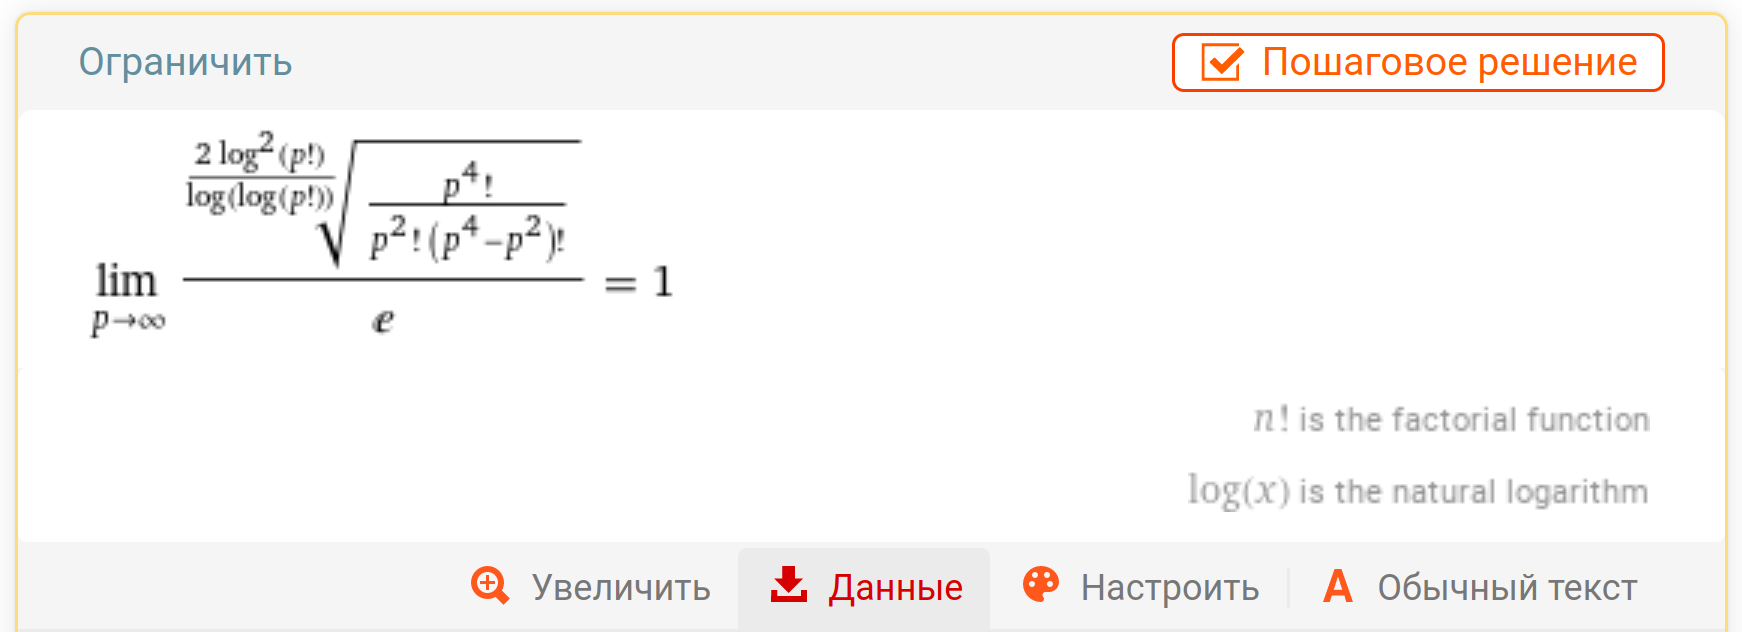
\includegraphics[scale=0.2]{Fall/img/solution-167_confirm.png}
\end{figure}

\textbf{Ответ: } \(\displaystyle f(s) = 2\frac{\ln{s}^2}{\ln{\ln{s}}}\).

\end{solution}

\begin{task}{449}
Пусть дана произвольная группа \(\mathbb{G}\) порядка \(\lvert\mathbb{G}\rvert = p^k,\, p\in\mathbb{P}\), докажите, что в \(\mathbb{G}\) имеется ровно \(p^m\) элементов \(a_i\) (для некоторого целого \(m>0\)), для каждого из которых его класс сопряжённости удовлетворяют равенству \(\left\lvert a_i^{\mathbb{G}}\right\rvert = 1\). В процессе решения кроме прочего вам может потребоваться доказать, что такое множество элементов образует подгруппу в \(\mathbb{G}\), также не помешает одно из следствий \emph{теоремы Лагранжа}.
\end{task}

\begin{solution}

\begin{enumerate}
    \item Если \(\left\lvert a^{\mathbb{G}}\right\rvert = 1\), то \(\forall g \in \mathbb{G}\:gag^{-1}=a \Leftrightarrow ag=ga\). Значит, \(a \in Z(\mathbb{G})\), а нам нужно доказать, что \(\left\lvert Z(\mathbb{G})\right\rvert = p^m\).

    \item Сопряжение~--- это отношение эквивалентности, разбивающее группу на непересекающиеся классы сопряженности, причем по теореме Лагранжа:
    \begin{equation*}
        \left\lvert a^{\mathbb{G}}\right\rvert = \frac{\left\lvert \mathbb{G}\right\rvert}{\left\lvert C_{\mathbb{G}}(a)\right\rvert},
    \end{equation*}
    другими словами, порядок класса сопряженности делит порядок группы.
    
    \item По прошлым пунктам мы можем утверждать, что:
    \begin{equation*}
        \left\lvert \mathbb{G}\right\rvert = \left\lvert Z(\mathbb{G})\right\rvert + \sum_i \left\lvert b_i^{\mathbb{G}}\right\rvert.
    \end{equation*}

    Сумма содержит не вошедшие в \(Z(\mathbb{G})\) элементы \(b_i\), то есть для каждого из них \(\left\lvert b_i^{\mathbb{G}}\right\rvert > 1\). А так как \(\lvert\mathbb{G}\rvert = p^k\) и порядок класса сопряженности делит порядок группы, получаем:
    \begin{equation*}
        \left\lvert \mathbb{G}\right\rvert = p^k = \left\lvert Z(\mathbb{G})\right\rvert + \sum_i p^{k_i}.
    \end{equation*}

    Получаем, что \(\left\lvert Z(\mathbb{G})\right\rvert\:\vdots\:p \Leftrightarrow \left\lvert Z(\mathbb{G})\right\rvert = p^m\), что и требовалось доказать.

\end{enumerate}

\end{solution}

\newpage
\begin{task}{468}
Найдите асимптотику количества различных раскрасок (необязательно правильных) графа на рисунке в \(k\) цветов  при \(k\to\infty\). Раскраски считаются одинаковыми, если они переходят друг в друга при некотором автоморфизме графа. Используйте теорему Редфилда\,--\,Пойи.
\end{task}

\begin{solution}

% Авточекер очень много ругается на tikz: он видит в "\node (1)" неправильное построение уравнения... 
% Бедное сочетание "Редфилда\,--\,Пойи", написание которого, между прочим, взято из условия, вообще "раздербанил" на несколько замечаний
% Синтаксически верное оформление предложения в строке 40 (двоеточие, тире) воспринял как правило сокращения порядковых числительных...
% В общем, авточекер прогнан, но он выворачивает действительность в обратную сторону. К сожалению, с библиотекой tikz он вообще не дружит. 

% Остальные замечания авточекера я исправил

Пронумеруем вершины графа и заметим симметрию при поворотах графа на \(90\) градусов:
\begin{figure}[H]
    \centering
    \tikz {
        \node (1) [circle, draw] at (2, 3) {1};
        \node (2) [circle, draw] at (3, 3) {2};
        \node (3) [circle, draw] at (3, 2) {3};
        \node (4) [circle, draw] at (2, 2) {4};
        \node (5) [circle, draw] at (2, 4) {5};
        \node (6) [circle, draw] at (3, 4) {6};
        \node (7) [circle, draw] at (4, 3) {7};
        \node (8) [circle, draw] at (4, 2) {8};
        \node (9) [circle, draw] at (3, 1) {9};
        \node (10) [circle, draw, scale=0.8] at (2, 1) {10};
        \node (11) [circle, draw, scale=0.8] at (1, 2) {11};
        \node (12) [circle, draw, scale=0.8] at (1, 3) {12};
        \node (sym1) at (2.5, 5) {};
        \node (sym2) at (2.5, 0) {};
        \node (sym3) at (0, 2.5) {};
        \node (sym4) at (5, 2.5) {};        
        
        \graph {
            (1) -- (2), (2) -- (3), (3) -- (4), (4) -- (1), (1) -- (3), (2) -- (4),
            (1) -- (5), (5) -- (6), (6) -- (2),
            (2) -- (7), (7) -- (8), (8) -- (3),
            (3) -- (9), (9) -- (10), (10) -- (4),
            (4) -- (11), (11) -- (12), (12) -- (1),

            (sym1) -- [dotted] (sym2), (sym3) -- [dotted] (sym4)
        };
    }
\end{figure}

В группе автоморфизмов, помимо тождественной перестановки, существуют три перестановки с поворотами вокруг центра тяжести \((1, 2, 3, 4)\) по часовой стрелке: \((1, 2, 3, 4)(5, 7, 9, 11)(6, 8, 10, 12)\). А также <<взгляд с обратной стороны>>: \\ \((1, 2)(3, 4)(5, 6)(7, 12)(8, 11)(9, 10)\),~--- и те же перестановки с поворотом по часовой стрелке на \(90\) градусов.

Получаем \(8\) автоморфизмов:
\begin{figure}[H]
    \centering
    \begin{subfigure}[b]{0.4\linewidth}
        \centering
        \tikz {
            \node (1) [circle, draw] at (2, 3) {1};
            \node (2) [circle, draw] at (3, 3) {2};
            \node (3) [circle, draw] at (3, 2) {3};
            \node (4) [circle, draw] at (2, 2) {4};
            \node (5) [circle, draw] at (2, 4) {5};
            \node (6) [circle, draw] at (3, 4) {6};
            \node (7) [circle, draw] at (4, 3) {7};
            \node (8) [circle, draw] at (4, 2) {8};
            \node (9) [circle, draw] at (3, 1) {9};
            \node (10) [circle, draw, scale=0.8] at (2, 1) {10};
            \node (11) [circle, draw, scale=0.8] at (1, 2) {11};
            \node (12) [circle, draw, scale=0.8] at (1, 3) {12};
            \node (sym1) at (2.5, 5) {};
            \node (sym2) at (2.5, 0) {};
            \node (sym3) at (0, 2.5) {};
            \node (sym4) at (5, 2.5) {};        
            
            \graph {
                (1) -- (2), (2) -- (3), (3) -- (4), (4) -- (1), (1) -- (3), (2) -- (4),
                (1) -- (5), (5) -- (6), (6) -- (2),
                (2) -- (7), (7) -- (8), (8) -- (3),
                (3) -- (9), (9) -- (10), (10) -- (4),
                (4) -- (11), (11) -- (12), (12) -- (1),
    
                (sym1) -- [dotted] (sym2), (sym3) -- [dotted] (sym4)
            };
        }
    \end{subfigure}
    \begin{subfigure}[b]{0.4\linewidth} 
        \centering
        \tikz {
            \node (1) [circle, draw] at (3, 3) {1};
            \node (2) [circle, draw] at (3, 2) {2};
            \node (3) [circle, draw] at (2, 2) {3};
            \node (4) [circle, draw] at (2, 3) {4};
            \node (5) [circle, draw] at (4, 3) {5};
            \node (6) [circle, draw] at (4, 2) {6};
            \node (7) [circle, draw] at (3, 1) {7};
            \node (8) [circle, draw] at (2, 1) {8};
            \node (9) [circle, draw] at (1, 2) {9};
            \node (10) [circle, draw, scale=0.8] at (1, 3) {10};
            \node (11) [circle, draw, scale=0.8] at (2, 4) {11};
            \node (12) [circle, draw, scale=0.8] at (3, 4) {12};
            \node (sym1) at (2.5, 5) {};
            \node (sym2) at (2.5, 0) {};
            \node (sym3) at (0, 2.5) {};
            \node (sym4) at (5, 2.5) {};        
            
            \graph {
                (1) -- (2), (2) -- (3), (3) -- (4), (4) -- (1), (1) -- (3), (2) -- (4),
                (1) -- (5), (5) -- (6), (6) -- (2),
                (2) -- (7), (7) -- (8), (8) -- (3),
                (3) -- (9), (9) -- (10), (10) -- (4),
                (4) -- (11), (11) -- (12), (12) -- (1),
    
                (sym1) -- [dotted] (sym2), (sym3) -- [dotted] (sym4)
            };
        }
    \end{subfigure}
    \begin{subfigure}[b]{0.4\linewidth} 
        \centering
        \tikz {
            \node (1) [circle, draw] at (3, 2) {1};
            \node (2) [circle, draw] at (2, 2) {2};
            \node (3) [circle, draw] at (2, 3) {3};
            \node (4) [circle, draw] at (3, 3) {4};
            \node (5) [circle, draw] at (3, 1) {5};
            \node (6) [circle, draw] at (2, 1) {6};
            \node (7) [circle, draw] at (1, 2) {7};
            \node (8) [circle, draw] at (1, 3) {8};
            \node (9) [circle, draw] at (2, 4) {9};
            \node (10) [circle, draw, scale=0.8] at (3, 4) {10};
            \node (11) [circle, draw, scale=0.8] at (4, 3) {11};
            \node (12) [circle, draw, scale=0.8] at (4, 2) {12};
            \node (sym1) at (2.5, 5) {};
            \node (sym2) at (2.5, 0) {};
            \node (sym3) at (0, 2.5) {};
            \node (sym4) at (5, 2.5) {};        
            
            \graph {
                (1) -- (2), (2) -- (3), (3) -- (4), (4) -- (1), (1) -- (3), (2) -- (4),
                (1) -- (5), (5) -- (6), (6) -- (2),
                (2) -- (7), (7) -- (8), (8) -- (3),
                (3) -- (9), (9) -- (10), (10) -- (4),
                (4) -- (11), (11) -- (12), (12) -- (1),
    
                (sym1) -- [dotted] (sym2), (sym3) -- [dotted] (sym4)
            };
        }
    \end{subfigure}
    \begin{subfigure}[b]{0.4\linewidth} 
        \centering
        \tikz {
            \node (1) [circle, draw] at (2, 2) {1};
            \node (2) [circle, draw] at (2, 3) {2};
            \node (3) [circle, draw] at (3, 3) {3};
            \node (4) [circle, draw] at (3, 2) {4};
            \node (5) [circle, draw] at (1, 2) {5};
            \node (6) [circle, draw] at (1, 3) {6};
            \node (7) [circle, draw] at (2, 4) {7};
            \node (8) [circle, draw] at (3, 4) {8};
            \node (9) [circle, draw] at (4, 3) {9};
            \node (10) [circle, draw, scale=0.8] at (4, 2) {10};
            \node (11) [circle, draw, scale=0.8] at (3, 1) {11};
            \node (12) [circle, draw, scale=0.8] at (2, 1) {12};
            \node (sym1) at (2.5, 5) {};
            \node (sym2) at (2.5, 0) {};
            \node (sym3) at (0, 2.5) {};
            \node (sym4) at (5, 2.5) {};        
            
            \graph {
                (1) -- (2), (2) -- (3), (3) -- (4), (4) -- (1), (1) -- (3), (2) -- (4),
                (1) -- (5), (5) -- (6), (6) -- (2),
                (2) -- (7), (7) -- (8), (8) -- (3),
                (3) -- (9), (9) -- (10), (10) -- (4),
                (4) -- (11), (11) -- (12), (12) -- (1),
    
                (sym1) -- [dotted] (sym2), (sym3) -- [dotted] (sym4)
            };
        }
    \end{subfigure}
    \caption{Повороты на 90 градусов.}
\end{figure}

\begin{figure}[H]
    \centering
    \begin{subfigure}[b]{0.4\linewidth}
        \centering
        \tikz {
            \node (1) [circle, draw] at (3, 3) {1};
            \node (2) [circle, draw] at (2, 3) {2};
            \node (3) [circle, draw] at (2, 2) {3};
            \node (4) [circle, draw] at (3, 2) {4};
            \node (5) [circle, draw] at (3, 4) {5};
            \node (6) [circle, draw] at (2, 4) {6};
            \node (7) [circle, draw] at (1, 3) {7};
            \node (8) [circle, draw] at (1, 2) {8};
            \node (9) [circle, draw] at (2, 1) {9};
            \node (10) [circle, draw, scale=0.8] at (3, 1) {10};
            \node (11) [circle, draw, scale=0.8] at (4, 2) {11};
            \node (12) [circle, draw, scale=0.8] at (4, 3) {12};
            \node (sym1) at (2.5, 5) {};
            \node (sym2) at (2.5, 0) {};
            \node (sym3) at (0, 2.5) {};
            \node (sym4) at (5, 2.5) {};        
            
            \graph {
                (1) -- (2), (2) -- (3), (3) -- (4), (4) -- (1), (1) -- (3), (2) -- (4),
                (1) -- (5), (5) -- (6), (6) -- (2),
                (2) -- (7), (7) -- (8), (8) -- (3),
                (3) -- (9), (9) -- (10), (10) -- (4),
                (4) -- (11), (11) -- (12), (12) -- (1),
    
                (sym1) -- [dotted] (sym2), (sym3) -- [dotted] (sym4)
            };
        }
    \end{subfigure}
    \begin{subfigure}[b]{0.4\linewidth}
        \centering
        \tikz {
            \node (1) [circle, draw] at (3, 2) {1};
            \node (2) [circle, draw] at (3, 3) {2};
            \node (3) [circle, draw] at (2, 3) {3};
            \node (4) [circle, draw] at (2, 2) {4};
            \node (5) [circle, draw] at (4, 2) {5};
            \node (6) [circle, draw] at (4, 3) {6};
            \node (7) [circle, draw] at (3, 4) {7};
            \node (8) [circle, draw] at (2, 4) {8};
            \node (9) [circle, draw] at (1, 3) {9};
            \node (10) [circle, draw, scale=0.8] at (1, 2) {10};
            \node (11) [circle, draw, scale=0.8] at (2, 1) {11};
            \node (12) [circle, draw, scale=0.8] at (3, 1) {12};
            \node (sym1) at (2.5, 5) {};
            \node (sym2) at (2.5, 0) {};
            \node (sym3) at (0, 2.5) {};
            \node (sym4) at (5, 2.5) {};        
            
            \graph {
                (1) -- (2), (2) -- (3), (3) -- (4), (4) -- (1), (1) -- (3), (2) -- (4),
                (1) -- (5), (5) -- (6), (6) -- (2),
                (2) -- (7), (7) -- (8), (8) -- (3),
                (3) -- (9), (9) -- (10), (10) -- (4),
                (4) -- (11), (11) -- (12), (12) -- (1),
    
                (sym1) -- [dotted] (sym2), (sym3) -- [dotted] (sym4)
            };
        }
    \end{subfigure}
    \begin{subfigure}[b]{0.4\linewidth}
        \centering
        \tikz {
            \node (1) [circle, draw] at (2, 2) {1};
            \node (2) [circle, draw] at (3, 2) {2};
            \node (3) [circle, draw] at (3, 3) {3};
            \node (4) [circle, draw] at (2, 3) {4};
            \node (5) [circle, draw] at (2, 1) {5};
            \node (6) [circle, draw] at (3, 1) {6};
            \node (7) [circle, draw] at (4, 2) {7};
            \node (8) [circle, draw] at (4, 3) {8};
            \node (9) [circle, draw] at (3, 4) {9};
            \node (10) [circle, draw, scale=0.8] at (2, 4) {10};
            \node (11) [circle, draw, scale=0.8] at (1, 3) {11};
            \node (12) [circle, draw, scale=0.8] at (1, 2) {12};
            \node (sym1) at (2.5, 5) {};
            \node (sym2) at (2.5, 0) {};
            \node (sym3) at (0, 2.5) {};
            \node (sym4) at (5, 2.5) {};        
            
            \graph {
                (1) -- (2), (2) -- (3), (3) -- (4), (4) -- (1), (1) -- (3), (2) -- (4),
                (1) -- (5), (5) -- (6), (6) -- (2),
                (2) -- (7), (7) -- (8), (8) -- (3),
                (3) -- (9), (9) -- (10), (10) -- (4),
                (4) -- (11), (11) -- (12), (12) -- (1),
    
                (sym1) -- [dotted] (sym2), (sym3) -- [dotted] (sym4)
            };
        }
    \end{subfigure}
    \begin{subfigure}[b]{0.4\linewidth}
        \centering
        \tikz {
            \node (1) [circle, draw] at (2, 3) {1};
            \node (2) [circle, draw] at (2, 2) {2};
            \node (3) [circle, draw] at (3, 2) {3};
            \node (4) [circle, draw] at (3, 3) {4};
            \node (5) [circle, draw] at (1, 3) {5};
            \node (6) [circle, draw] at (1, 2) {6};
            \node (7) [circle, draw] at (2, 1) {7};
            \node (8) [circle, draw] at (3, 1) {8};
            \node (9) [circle, draw] at (4, 2) {9};
            \node (10) [circle, draw, scale=0.8] at (4, 3) {10};
            \node (11) [circle, draw, scale=0.8] at (3, 4) {11};
            \node (12) [circle, draw, scale=0.8] at (2, 4) {12};
            \node (sym1) at (2.5, 5) {};
            \node (sym2) at (2.5, 0) {};
            \node (sym3) at (0, 2.5) {};
            \node (sym4) at (5, 2.5) {};        
            
            \graph {
                (1) -- (2), (2) -- (3), (3) -- (4), (4) -- (1), (1) -- (3), (2) -- (4),
                (1) -- (5), (5) -- (6), (6) -- (2),
                (2) -- (7), (7) -- (8), (8) -- (3),
                (3) -- (9), (9) -- (10), (10) -- (4),
                (4) -- (11), (11) -- (12), (12) -- (1),
    
                (sym1) -- [dotted] (sym2), (sym3) -- [dotted] (sym4)
            };
        }
    \end{subfigure}
    \caption{Повороты на 90 градусов, <<взгляд с обратной стороны>>.}
\end{figure}

По теореме Редфилда\,--\,Пойи, асимптотика количества различных раскрасок графа на \(n\) вершинах \(k\) цветов при \(k\to\infty\) есть:
\begin{equation*}
    \frac{k^n}{\left\lvert Aut \right\lvert} = \frac{k^{12}}{8}.
\end{equation*}

\textbf{Ответ: } \(\displaystyle \frac{k^{12}}{8}\).

\end{solution}

\newpage
\begin{task}{191}
Дана последовательность \(a_n\), заданная линейным рекуррентным соотношением \(a_{n+3}+a_{n+2}-16a_{n+1}+20a_n=0\) при условии, что \(a_0=4, a_1=2, a_2=20\). Вычислите значение выражения \(\sum_{n=0}^{+\infty}na_n\left(\frac{1}{10}\right)^n\), используя <<свёртку>> производящей функции.
\end{task}

\begin{solution}

Найдем <<свёртку>> производящей функции:
\begin{gather*}
    G(z) = a_0 + a_1z + a_2z^2 + \sum_{n=3}^{\infty} \left(-a_{n-1} + 16a_{n-2} - 20a_{n-3} \right)z^n = \\
    = a_0 + a_1z + a_2z^2 - z\sum_{n=2}^{\infty} a_nz^n + 16z^2\sum_{n=1}^{\infty} a_nz^n - 20z^3\sum_{n=0}^{\infty} a_nz^n = \\
    = a_0 + a_1z + a_2z^2 - z\left(G(z) - a_0 - a_1z \right) + 16z^2\left(G(z) - a_0 \right) - 20z^3G(z) = \\
    = 4 + 2z + 20z^2 - z\left(G(z) - 4 - 2z \right) + 16z^2\left(G(z) - 4 \right) - 20z^3G(z) = \\
    = G(z)(-z + 16z^2 - 20z^3) + 4 + z\left(2 + 4 \right) + z^2\left(20 + 2 - 16 \cdot 4 \right) = \\
    = G(z)(-z + 16z^2 - 20z^3) + 4 + 6z - 42z^2.
\end{gather*}

В итоге находим \(G(z) = \frac{4 + 6z - 42z^2}{1 + z - 16z^2 + 20z^3}\).

Если ряд представить суммой, то:
\begin{equation*}
    G(z) = \sum_{n=0}^{\infty} a_nz^n \Rightarrow \sum_{n=0}^{\infty} na_nz^n = z \cdot G'(z).
\end{equation*}

Обозначим \(P(z) = z \cdot G'(z)\). Тогда \(P(0.1)\) даст требуемый ответ. Однако следует проверить сходимость \(P(z)\) при \(z = 0.1\). Если радиус сходимости этого ряда, соответствующий в нашем случае наименьшему по модулю корню знаменателя \(G(z)\), окажется больше \(z = 0.1\), тогда ряд сходится. В таком случае нам нужно удостовериться, что:
\begin{equation*}
    \left(\forall x \in \left[-\frac{1}{10}; \frac{1}{10} \right] \right) T(x) = 1 + x - 16x^2 + 20x^3 \neq 0.
\end{equation*}

Найдем производную \(T(x)\), её корни, отсюда границы возрастания и убывания самой функции и определим, есть ли нули у \(T(x)\) на отрезке \([-0.1; 0.1]\):
\begin{equation*}
    T'(x) = 60x^2 - 32x^2 + 1 = (30x - 1)(2x - 1); \: T(\frac{1}{30}) = \frac{254}{250}.
\end{equation*}

Отсюда:
\begin{align*}
    \text{Возрастает на } [-\frac{1}{10}; \: &\frac{1}{30}]; T(-\frac{1}{10}) = \frac{18}{25}, \\
    \text{Убывает на } [\frac{1}{30}; \: &\frac{1}{10}]; T(\frac{1}{10}) = \frac{24}{25}.
\end{align*}

Исходя из промежутков возрастания и убывания функции, а также её значений в крайних точках \([-0.1; 0.1]\), делаем вывод, что на отрезке функция \(T(x)\) никогда не обращается в ноль. Следовательно, радиус сходимости больше \(0.1\), и ряд \(P(x)\) в этой точке будет сходится. Найдем его значение:
\begin{gather*}
    P(z) = z \cdot G'(z) = z \cdot \frac{420z^3 + 90z^2 - 48z - 2}{(1 + z - 16z^2 + 20z^3)^2}; \\
    P(\frac{1}{10}) = \frac{1}{10} \cdot \frac{-5.48}{0.9216} = -\frac{685}{1152}.
\end{gather*}

\textbf{Ответ:} \(\displaystyle -\frac{685}{1152}\).

\end{solution}

\begin{task}{356}
При каких \(k,n,t\) будет заведомо существовать система различных представителей для совокупности из \(t\) различных \(k\)-элементных подмножеств \(n\)-элементного множества? А при каких \(k,n,t\) с.\,р.\,п. заведомо не будет существовать?
\end{task}

\begin{solution}

При решении задачи будем пользоваться следствием теоремы Холла:
\begin{corollary}\label{corollary_Hall}
Система различных представителей для семейства подмножеств \(\{A_1, \ldots, A_s\}\) существует тогда и только тогда, когда объединение \(m\::\:\left( 1 \leqslant m \leqslant s \right)\) множеств \(A_i\) содержит не менее \(m\) элементов.
\end{corollary}

Во-первых, заметим, что \(C_{k + 1}^{k} = k + 1\), то есть объединение \(k + 1\) различных \(k\)-элементных подмножеств будет содержать по крайней мере \(k + 1\) элемент. По следствию~\ref{corollary_Hall} система различных представителей будет существовать. Этим мы выделяем \emph{существование с.\,р.\,п. при \(t = k + 1, n \geqslant k + 1\)}. Каждое подмножество \(k\)-элементное, \(k \leqslant |\cup A_i|\), значит, для любого \(1 \leqslant m \leqslant s = k\), \emph{то есть при \(t < k + 1\), с.\,р.\,п. также найдется}.

Приведем пример с условием \(t > k + 1\), где с.\,р.\,п. не будет существовать.

Пусть \(n \geqslant k + 2, s = k + 2\). Возьмем \(k + 1\) различных \(k\)-элементных подмножеств, объединение которых будет содержать ровно \(k + 1\) элемент. Добавим к ним еще одно множество, в котором будет присутствовать \(k + 2\) элемент, не содержащийся в остальных \(k + 1\) подмножествах. Тогда по следствию~\ref{corollary_Hall} при \(1 \leqslant m = k + 1 \leqslant s = k + 2\) объединение первых \(k + 1\) подмножеств должно содержать не менее \(k + 2\) элементов, однако это не так. Данное противоречие позволяет нам утверждать, что \emph{при \(t > k + 1, n \geqslant k + 2\) с.\,р.\,п. не существует}.

Так мы определили, что \textbf{при \(\left(t \leqslant k + 1, n \geqslant t\right)\) с.\,р.\,п. всегда найдется}.

Дополнительно в рассуждениях мы всегда отмечали, что \(n \geqslant t\). Действительно, если \(n < t\), тогда объединение \(t\) различных \(k\)-элементных подмножеств таково, что его мощность обязательно будет не больше \(n\), значит, вместе с тем меньше \(t\), что противоречит следствию~\ref{corollary_Hall}:
\begin{equation*}
    t = |\cup A_i| \leqslant n < t.
\end{equation*}

Таким образом:
\begin{enumerate}
    \item с.\,р.\,п. заведомо существует при \(t \leqslant k + 1, n \geqslant t\);
    
    \item с.\,р.\,п. заведомо не будет существовать при \(n < t\).
\end{enumerate}

\end{solution}

\begin{task}{376}
Целое число \(x\) называется \emph{квадратичным вычетом} по модулю \(m\), если \((x, m)=1\) и существует такое целое \(y\), что \(x \equiv y^2 \pmod{m}\). Пусть даны попарно взаимно простые числа \(m_1,m_2,\dots,m_n\in \mathbb{N}\) и \(M=\prod_{i=1}^n m_i\). Используя китайскую теорему об остатках (необязательно использовать явный вид решения, достаточно существования и единственности), докажите, что \(x\) является квадратичным вычетом по модулю \(M\) тогда и только тогда, когда \(x\) является таковым по каждому модулю \(m_i\). 

\textbf{Техническое требование:} при оформлении запишите формулировку теоремы, которой будете пользоваться, с помощью окружения \emph{theorem}.
\end{task}

\begin{solution}

Ниже приведена формулировка Китайской теоремы об остатках (КТО):
\begin{theorem}\label{theorem_CRT}
Если натуральные числа \(m_{1}, m_{2}, \dots, m_{n}\) попарно взаимно просты, то для любых целых \(r_{1}, r_{2}, \dots, r_{n}\) таких, что \(0 \leqslant r_{i} < m_{i}\) при всех \(i \in \{1, 2, \dots, n\}\), найдётся число \(M\), которое при делении на \(m_{i}\) даёт остаток \(r_{i}\) при всех \(i \in \{1, 2, \dots, n\}\). Более того, если найдутся два таких числа \(M_1\) и \(M_2\) (соответствующих утверждению выше), то \(M_{1} \equiv M_{2}{\pmod  {m_{1} \cdot m_{2} \cdot \ldots \cdot m_{n}}}\).
\end{theorem}

\textbf{Докажем в правую сторону \((\Rightarrow)\)}.

Если \(x\) является квадратичным вычетом \(M\), то \(x\) также является квадратичным вычетом \(m_i \left(1 \leqslant i \leqslant n \right)\), так как каждый \(m_i \: | \: M\).

\textbf{Докажем в обратную сторону \((\Leftarrow)\)}.

Пусть \(x \equiv y_i^2 \pmod{m_i} \left(1 \leqslant i \leqslant n \right)\). Используя КТО (Теорема~\ref{theorem_CRT}), обнаружим:
\begin{equation*}
    \exists! \: K: \: \left(1 \leqslant i \leqslant n \right) \left[ K \equiv y_i \pmod{m_i} \Rightarrow K^2 \equiv y_i^2 \equiv x \pmod{m_i} \right]. 
\end{equation*}

Используя ту же КТО (Теорема~\ref{theorem_CRT}), точнее, часть о единственности, находим, что \(K^2 \equiv y_i^2 \equiv x \pmod{m_i} \Rightarrow x \equiv K^2 \pmod{M}\).

Осталось проверить, что выполняется условие:
\begin{equation*}
    \left[ \forall \left(1 \leqslant i \leqslant n \right) (x, m_i) = 1 \right] \Leftrightarrow (x, M) = 1.
\end{equation*}

Оно, очевидно, справедливо ввиду взаимной простоты всех \(m_i\) между собой и с числом \(x\).

\end{solution}

\begin{task}{401}
Пусть дана последовательность различных натуральных чисел длины \(k^4+1\). \textbf{Используя теорему Мирского или теорему Дилуорса}, докажите, что в этой последовательности можно выделить либо подпоследовательность длины \(k+1\), в которой каждое следующее число \emph{делится} на предыдущее, либо подпоследовательность длины \(k+1\), в которой каждое следующее число \emph{делит} предыдущее, либо монотонную подпоследовательность длины \(k+1\), в которой любые два числа не являются делителями друг друга. \textbf{При решении нужно обязательно оформить формулировку используемой теоремы с помощью окружения \emph{theorem}, а также сослаться на неё при помощи команды \emph{ref}}.
\end{task}

\begin{solution}

\begin{theorem} [Теорема Дилуорса] \label{Dilworth}
    Наименьшее количество цепей, покрывающих конечное ЧУМ, равно наибольшему размеру антицепи в этом ЧУМе.
\end{theorem}

Зададим на последовательности длины \(k^4+1\) строгий частичный порядок \(\prec\):
\begin{equation*}
    \left( a_i \prec a_j \right) \equiv \left( a_i < a_j \land i < j \right).
\end{equation*}
Это отношение порядка позволяет установить, образуют ли выбранные элементы монотонную подпоследовательность. В том числе, если \(a \prec b\), тогда \(\left( a, b \right)\)~--- монотонно возрастающая подпоследовательность. В противном случае это монотонно убывающая подпоследовательность, так как числа последовательности различные.

Заметим также, что элементы, образующие цепь, также формируют монотонно возрастающую последовательность. Аналогично антицепь является монотонно убывающей последовательностью.

Так в последовательности \(\left( 1, 8, 2, 6, 5, 4, 7 \right)\) можно выделить монотонно возрастающую подпоследовательность \(\left( 1, 2, 4, 7 \right)\), а также монотонно убывающую подпоследовательность \(\left( 8, 5, 4 \right)\).

Вместе с порядком \(\prec\) последовательность длины \(k^4+1\) становится ЧУМ, и теперь можно применить Теорему Дилуорса~\ref{Dilworth}:
\begin{enumerate}
    \item Если нашлась антицепь размера \(k^2+1\), тогда мы нашли монотонно \emph{убывающую} подпоследовательность;
    
    \item Если же наибольший размер антицепи меньше \(k^2+1\), значит, можно найти покрытие ЧУМа размера \(k^4+1\) не более чем \(k^2\) цепями, и, используя метод Дирихле, делаем вывод, что среди них обязательно найдется цепь длины не меньше \(k^2+1\)~--- то есть мы нашли монотонно \emph{возрастающую} подпоследовательность.
\end{enumerate}

В любом случае выявится монотонная подпоследовательность длины \(k^2+1\). Снова применяем теорему Дилуорса~\ref{Dilworth} для ЧУМа, получившегося из новой теперь уже \emph{монотонной} последовательности длины \(k^2+1\), но с новым порядком делимости |:
\begin{enumerate}
    \item Если наибольший размер антицепи меньше \(k+1\), значит, можно найти покрытие ЧУМа размера \(k^2+1\) не более чем \(k\) цепями, и, используя метод Дирихле, делаем вывод, что среди них обязательно найдется цепь длины не меньше \(k+1\). Тогда:
    \begin{enumerate}
        \item Если нашлась цепь размера \(k+1\) в \emph{монотонно убывающей} последовательности длины \(k^2+1\), тогда мы нашли искомую \emph{подпоследовательность длины \(k+1\), в которой каждое следующее число делится на предыдущее};

        \item Если нашлась цепь размера \(k+1\) в \emph{монотонно возрастающей} последовательности длины \(k^2+1\), тогда мы нашли искомую \emph{подпоследовательность длины \(k+1\), в которой каждое следующее число \emph{делится} на предыдущее};
    \end{enumerate}
    
    \item В противном случае найдется антицепь размера \(k+1\) в \emph{монотонной} последовательности длины \(k^2+1\), значит, мы нашли искомую \emph{монотонную подпоследовательность длины \(k+1\), в которой любые два числа не являются делителями друг друга}.
\end{enumerate}

Таким образом, условие задачи выполнено.

\end{solution}

\end{document}
